\documentclass[11pt]{article}

\usepackage[margin=0.75in]{geometry}
\usepackage{url}
\usepackage{graphicx}
\usepackage{float}
\usepackage{amsmath}
\usepackage[utf8]{inputenc}
\PassOptionsToPackage{usenames,dvipsnames,svgnames}{xcolor}  
\usepackage{tikz}
\usetikzlibrary{arrows,positioning,automata}
\graphicspath{ {figs/} }

\title{An Analysis of fcMRI data in Schizophrenia}
\author{
  Hejazi, Nima\\
  \texttt{nhejazi}
  \and
  Lin, Feng\\
  \texttt{LiamFengLin}
  \and
  Zhao, Luyun\\
  \texttt{lynnzhao92}
  \and
  Zhou, Xinyue\\
  \texttt{z357412526}
}

\bibliographystyle{siam}

\begin{document}
\maketitle

\abstract{We report analyses intended to explore the functional magnetic
  resonance imaging (fMRI) data collected in studies conducted by Repovs et al.,
on the manner in which brain network connectivity is related to schizophrenia
\cite{repovs2011,repovs2012}. A host of exploratory techniques, as well as
linear modeling and brain network connectivity analyses across 20 subjects, were 
used in order to gain further insights into the fMRI data examined.}

\section{Introduction}

The human central nervous system is a complex dynamic network, consisting of
numerous functional regions that coordinate everything from simple reflexes to
complicated thoughts. In an effort to better understand the manner in which
functional changes contribute to the symptoms of schizophrenia, Repovs \textit{et
al.} conducted neuroimaging studies, including both functional connectivity
magnetic resonance imaging (fcMRI) and diffusion tensor imaging (DTI), on 102
subjects. The goal was to characterize the activity of several brain
regions that were chosen \textit{a priori}, and to develop an understanding of how 
the functional activities of these regions may differ across health states \cite{repovs2011,repovs2012}.

For the main analysis, we focused on Generalized Linear Model and Connectivity analysis as outlined below. Besides these main analyses, we performed various exploratory data analyses (EDA), such as finding root mean square (RMS) outliers, K-Means clustering, correlations with different baseline functions that helped us understand the data. The details of the EDA and relevant discussion of the results can be found in the appendix. 

\subsection{Generalized Linear Model}

The goal of GLM with respect to our dataset is to detect the activation clusters of target and non-target events in one subject in the control (healthy) group. An activation cluster refers to a group of neighboring voxels activated beyond certain statistical thresholds (e.g., t-test, t-values) by defined events. We did not set up a quantifiable criterion -- for example, to definitively separate one cluster from a neighboring cluster, but provide qualitative evidence in terms of coefficient and t-value maps. Please see the methods section that follows for the target and non-target events definitions. 

GLM is performed for both 0-back and 2-back tasks for the subject so that we can assess the effect of different memory loads on activation clusters. Through the GLM, we are better able to access the noise structure of the data, so that we can remove the noise regressors as a step towards a connectivity analysis. 

\subsection{Connectivity Analysis}

We are interested in the neural responses of the schizophrenic patients in a memory-related task, compared to the healthy controls. The goal of connectivity analysis is to compare the functional brain connectivity, measured by ROI-ROI correlations of 2-back task data between the four networks of the brain (DMN, FP, CO, CER), across controls (referred to as CON and composed of members of the control group and their siblings) and schizophrenics (referred to as SCZ and composed of patients with schizophrenia and their siblings) \footnote{The consideration behind such grouping is that in general, participants share similar brain structure and functions with their siblings, regardless of whether they have developed schizophrenia.}. The task data was pre-precessed by removing the noise regressors after fitting the GLM described above. The four aforementioned networks are thought to be critical for cognitive function, as defined in the paper: (1) default mode network (DMN); (2) dorsal fronto-parietal network (FP); (3) cingula-opercular network (CO); (4) cerebellar network (CER) \cite{repovs2012}. We restrict our focus to the 2-back task because it is the most cognitively difficult to perform amongst the three levels of the n-back tasks and requires the highest memory load, thus making it more likely to reveal the differences of the response of the brains of the patients versus those of the controls.

\section{Data}

The analyses reported in this paper are based on data generated in a series of
neuroimaging experiments conducted by Barch, Repovs, \& Csernansky. The aim of
these experiments was to ascertain the activity of several brain networks
thought to be associated with depressed cognitive function in individuals with
schizophrenia by collecting functional connectivity magnetic resonance imaging
(fcMRI) data on healthy individuals, individuals with schizophrenia, and the
(healthy) siblings of participants in either of the two former groups
\cite{repovs2012}. For the purposes of the analyses reported in this paper, the imaging
data were acquired from the OpenfMRI project (\url{https://openfmri.org/}), where they
are listed with accession number ds115. The data is available for groups of
subjects, with each subject-specific data directory containing anatomical MR
imaging data, functional MR imaging (using the BOLD contrast) data, and
diffusion tensor imaging (DTI) data. A n-back task was conducted during which the
subject was asked to identify whether the current letter is the same as the 
nth preceeding letter. Note that for 0-back, the 0th preceeding letter is 
pre-specificed before the run instead of being presented continuously throughout the run. 


\section{Methods}

\subsection{Data Preprocessing}

The standard preprocessed BOLD images were used for all analyses. They were already preprocessed with (1) motion correction (co-registration in time to partially correct for movement during the run and between runs); (2) temporary high-pass filtering to remove low frequency drifts and/or noise; and (3) registration to a standard anatomical template (the MNI template). In EDA, we detected several extended root-mean-square (RMS) outliers for the raw BOLD datasets. This justified the need for temporary smoothing as one of the reasons to use the standard preprocessed data. 

For our preprocessing steps, first five images of each run were removed to allow measurements to achieve steady state. Each image was passed through a gaussian filter of $\sigma=2$. This spatial smoothing approach assumes that fMRI data inherently show spatial correlations due to functional similarities of adjacent brain regions. To address the fact that boundary voxels of the brain were smoothed with measurements outside the brain, we implemented substitution of voxels near but outside the boundaries of brain with neighboring measurements within the boundary of the brain. However, this was not applied to connectivity portion of the analysis because the implementation was very slow and would take several hours on 20 subjects.

\subsection{Data Analysis}

\subsubsection{Generalized Linear Model}

Before proceeding to discussions of the specifics of our GLM approach, we believe it worthwhile to discuss the details of the condition files in the dataset because we make use of all condition files in the GLM. A major problem we encountered was that the keys in the metadata folder of the dataset that was provided does not correspond to the condition files, so the keys and the related descriptions of the condition files are redefined as given below. 

\begin{itemize}

\item cond001: Start cues for both blocks of the run.

\item cond002: The visual stimuli (i.e. letters) presenteed to the subject. The
intensities are all one because there is only one homogeneous event type.

\item cond003: The target and non-target events during the run. A target is the event
that the current letter that is the same as the nth preceeding letter. A non-target is the opposite
of a target, in which the current letter is not the same. 

\item cond004: Done cues for both blocks of the run.

\item cond005: Start and durations of the two blocks with a rest (i.e. fixation)
period in between the blocks. This is different from resting-state data, which
is mentioned in the reference papers but is not included on the OpenfMRI
website. 

\item cond006: This is unknown and is not explained in the paper.

\item cond007: Errors made by the subject when responding for each letter shown
whether it was the same as a pre-specified (0-back) or preceding (1,2-back)
letter.

\end{itemize}

We now proceed to describing the regressors in the GLM on each voxel time
course. For all convolutions below, a specified condition on-off time course 
file was convolved at a time unit of 0.01 TR with a gamma function and take the
convolved values at the start of each TR. After outlineing the regressors, one 
of the design matrix is shown in Figure 2 below. Additionally, in order to show
that the noise regressors are not trivial, a graph displaying fit for thses regressors 
are included in the appendix. 

\begin{itemize}
\item reg001: Convolution of target events from cond003. Essentially, we split cond003
into separate regressors, target and non-target with the assumption that they
different in the levels of activitities.

\item reg002: Convolution of non-target events from cond003.

\item reg003: Convolution of error events from cond007.

\item reg004: On-off time course from cond005. This regressor is included to account
for mean differences in the two blocks of the same run.

\item reg005: Convolution of start cues from cond001. This is separated from the
target and non-target regressors in that it is not part of tasks and that it is
not likely to involve heavy working memory load as tasks.

\item reg006: Convolution of done cues from cond004. It has the same purpose as
reg005.

\item reg007 and reg008: A linear drift term and a quadratic drift term included as
potential nuisansance regressors. Their significance is investigated below.

\item reg009 and reg010: The first two Principal Components of the data. Based on the
projections shown in Figure 1 below, we decide that the first two are not functional
features.

\item reg011: Intercept term.

\end{itemize}

\begin{figure}[H]
\centering
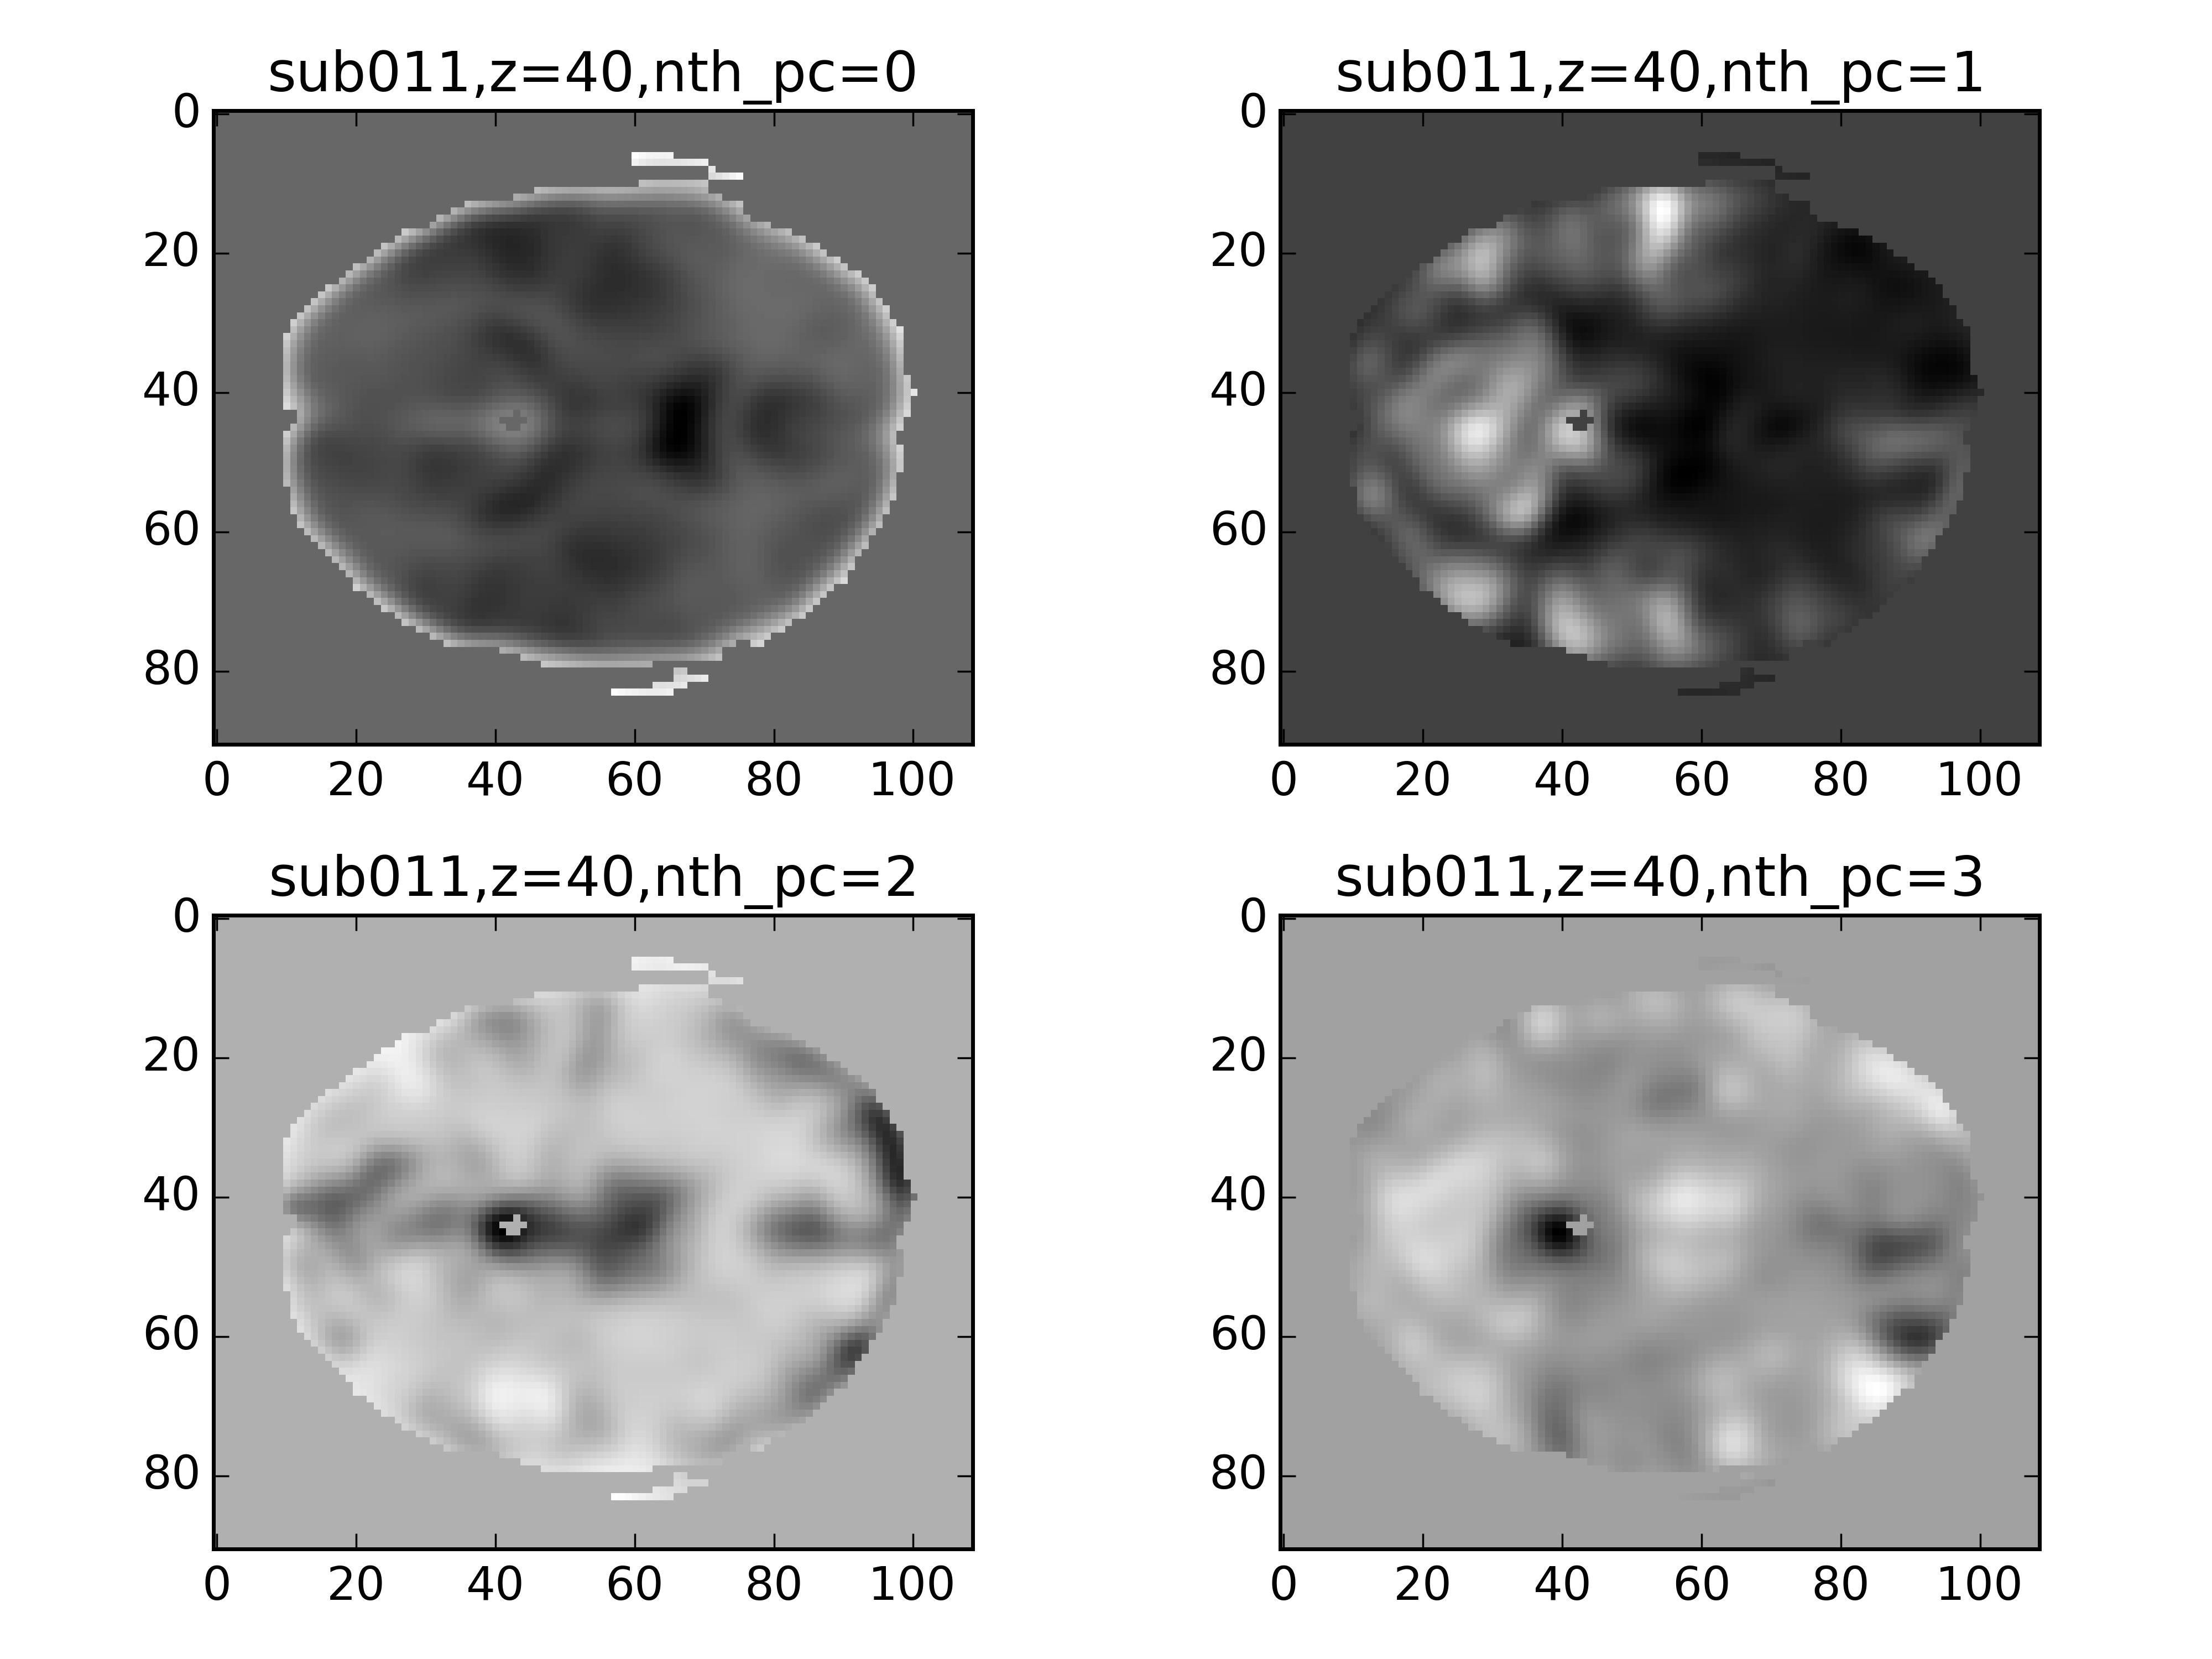
\includegraphics[scale=0.4]{../results/sub011_task001_first_four_pcs.png}
\caption{The first four Principal Components (pc) for sub011, 0-back.}
\end{figure}

\begin{figure}[H]
\centering
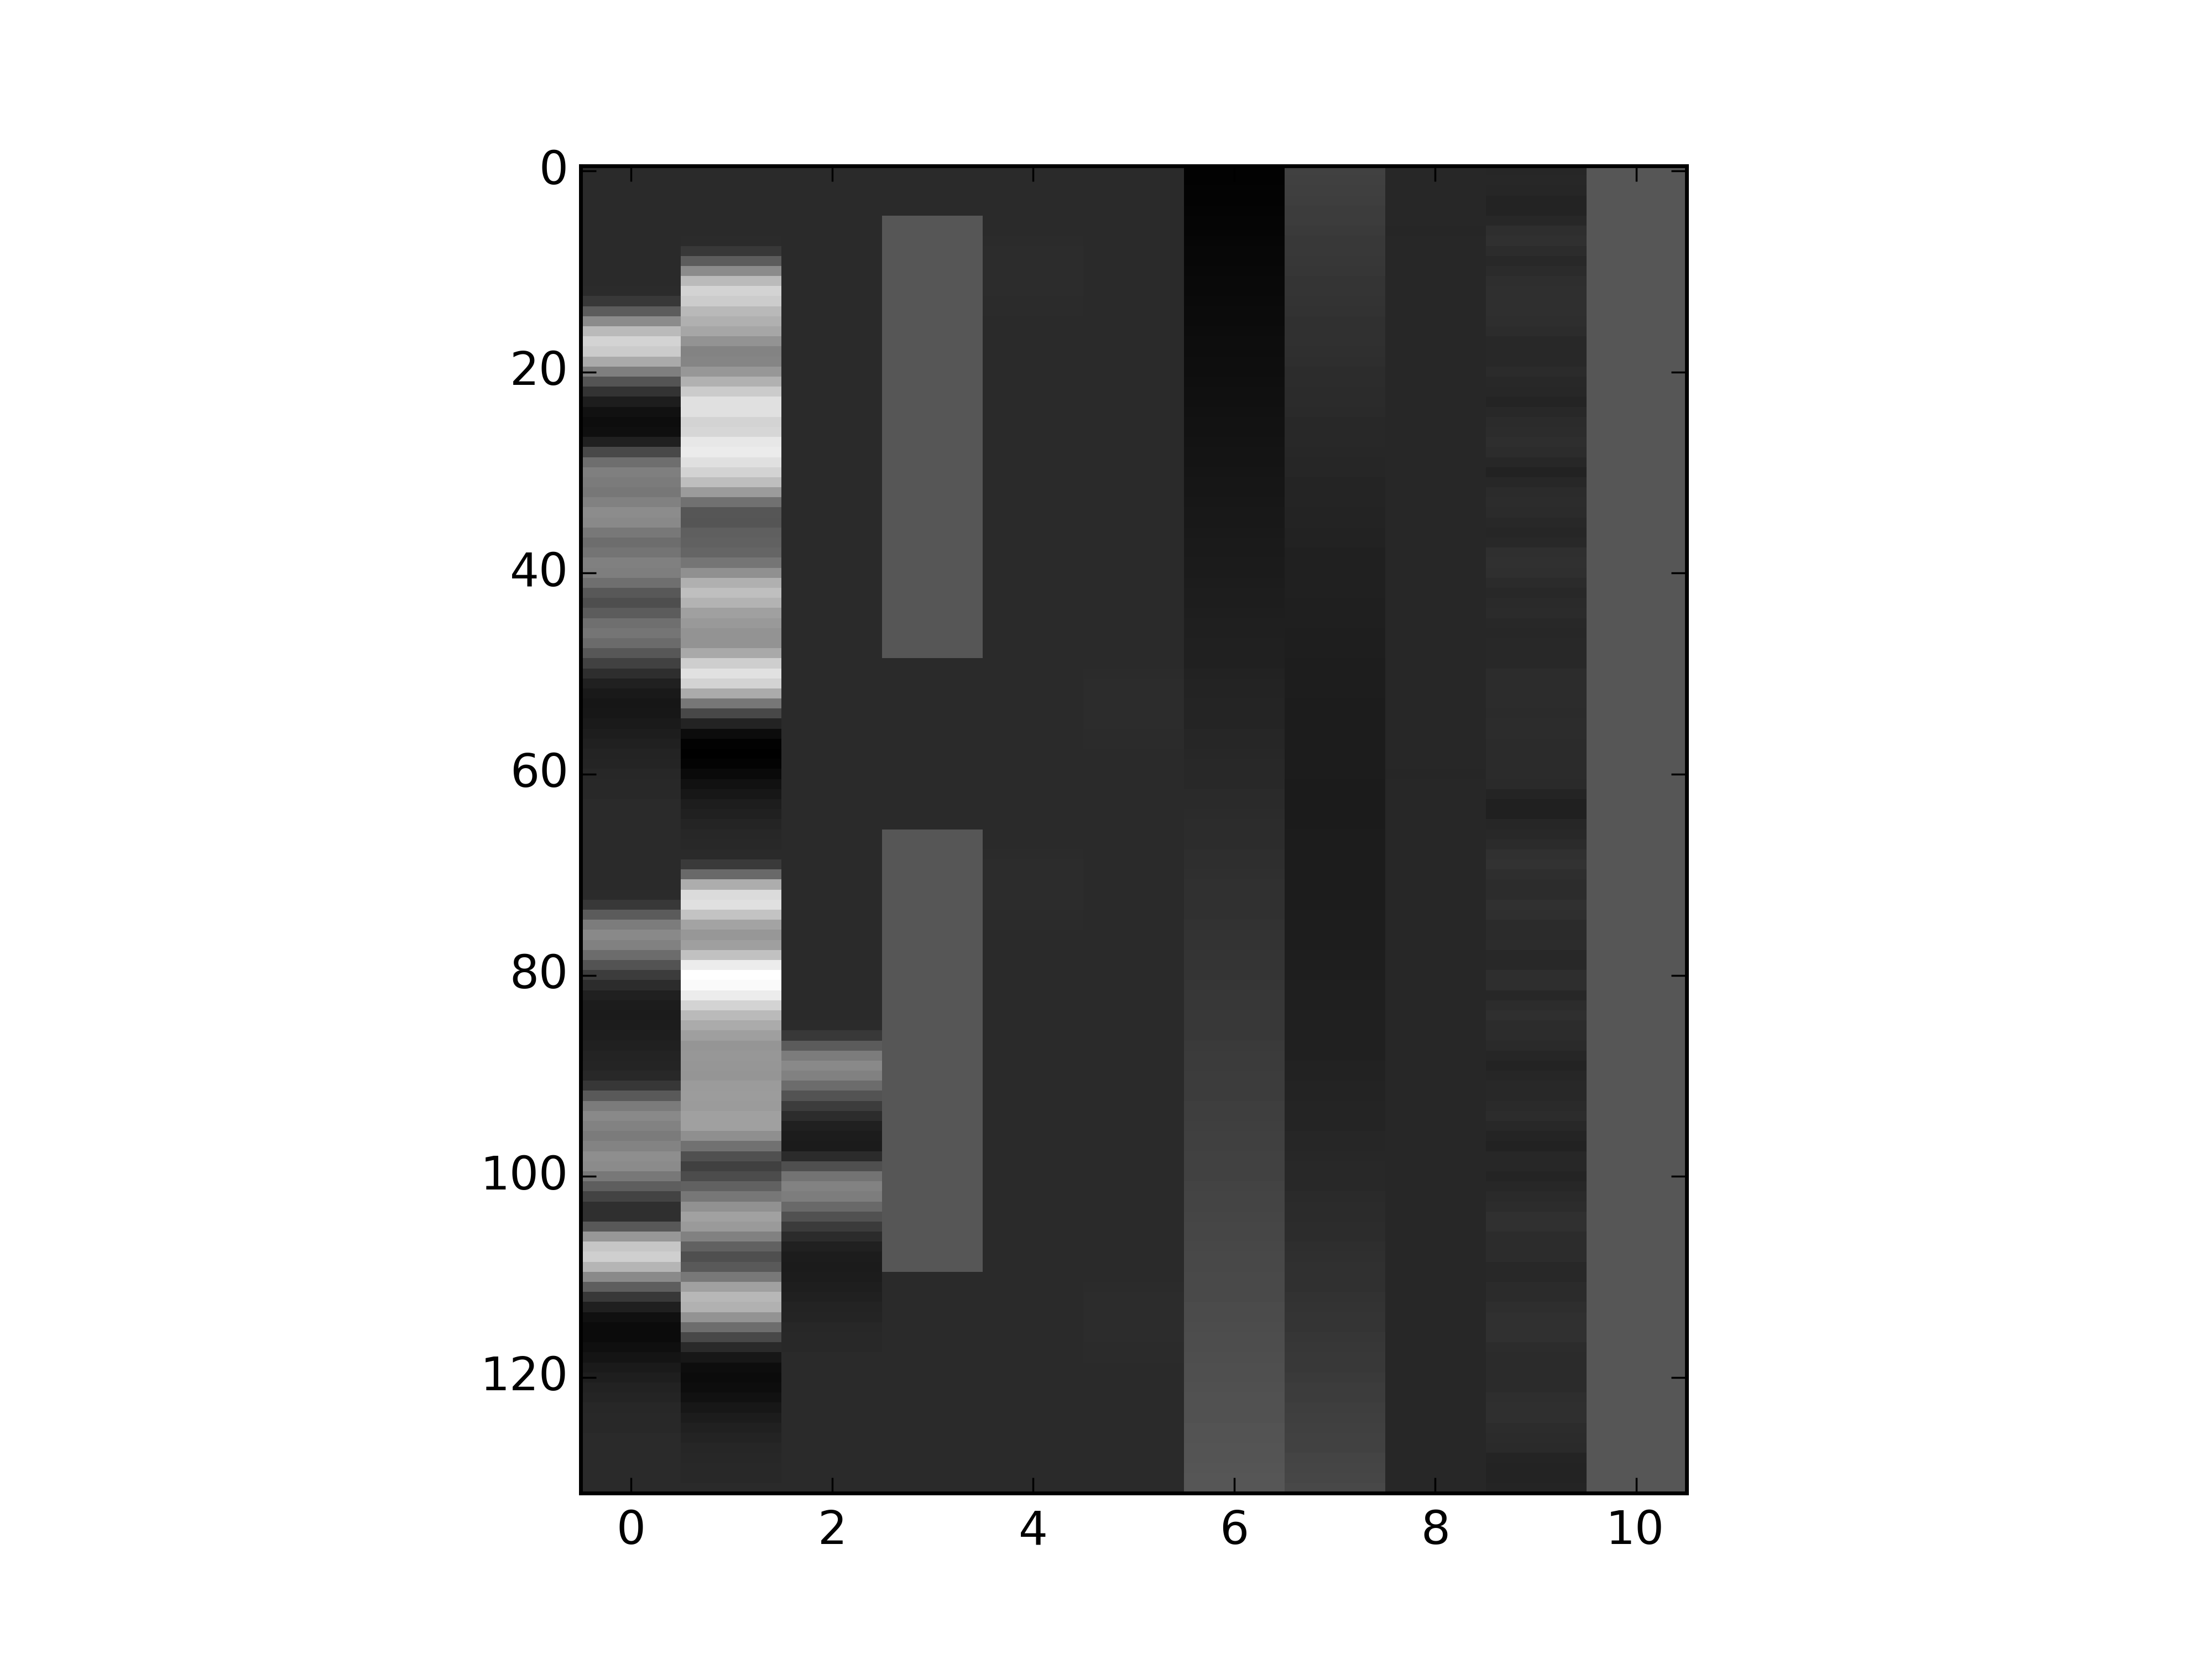
\includegraphics[scale=0.4]{../results/sub011_task003_design_matrix.png}
\caption{The design matrix for subject 011, 2-back. The indices correspond to the regressors
from reg001 to reg011. Index 4 and 5 are almost unidentifiable from the graph because they
are convolved from only a few single neural prediction values and hence are very small.}
\end{figure}

For each $\beta$ on each voxel time course, a linear regression of two-tailed
t-test is conducted to access whether there is a significant linear relationship
between the dependent variable Y and the regressor associated with the $\beta$,
with significance levels of 0.05 for each test. \\
 
\textit{Null Hypothesis}: $ \beta = 0$ \\

\textit{Alternative Hypothesis}: $\beta \neq 0$ \\

Instead of plotting out the regions of siginificant p-values, the t-value map of
the entire brain is presented within the results section that follows. 

Before performing t-tests, we assess the validity of t-tests by examining its
assumptions. The two main assumptions are (1) the residuals of each linear model
are independent and identically distributed (i.i.d), and (2) residuals for the model
are normally distributed. The Shapiro-Wilk test is performed on the residuals of
each voxel time course in the linear model. 37703 out of 207766 voxels fail this
test; however, when performing a large number of statistical tests, some may have
p-values less than 0.05 purely by chance (that is, it now becomes necessary to control the false discovery rate). To test the normality of several models together, three multiple comparison tests (namely, Bonferroni, Hochberg, and Benjamini-Hochberg), were performed, and results are shown below \footnote{The results were generated from our analysis scripts, and can be found in the results folder at \textit{sub011\_task003\_linear\_model\_normality\_test\_failure\_rates.csv}}. \\

\textit{Bonferroni}: normality assumption is violated in 6 voxels. \\

\textit{Hochberg}: normality assumption is violated in 262 voxels. \\

\textit{Benjamini-Hochberg}: all of voxels pass the normality test. \\

In summary, we can conclude that our assumption of normality in the residuals is
generally valid and hence can proceeed to perform t-test.

\subsubsection{Connectivity Analysis}

The roadmap for the analytic steps followed to examine connectivity is as
follows:

\begin{enumerate}
  \item Removal of noise regressors from the voxel time series: Linear model as
    defined in the GLM section was fitted to two BOLD runs (0-back and 2-back) across 20 subjects.
    The residuals  after removal of the noise regressors (i.e. reg004 to reg011 
    listed in the GLM section) were the input time series to the steps that follows.
  \item Extraction of voxels per region of interest (ROI): ROIs of the four
    networks respectively are defined by a center and a diameter as 15mm \cite{repovs2012}. Two 
    validations are made before the analysis: (1) it is ensured that the ROIs are 
    non-overlapping by setting the diameters for each ROI sphere as less than 
    the minimum distance between any two given ROIs in the full set, and 
    (2) ROIs are represented as spheres instead of cubes in order to better 
    approximate the underlying neurobiology and to make computing minimum distances 
    between the ROIs straitforward.
  \item In order to compute the ROI-ROI correlations, several steps were
    taken: (1) for each ROI in a given network, the corresponding voxels in the defined
    sphere were extracted and their time series were averaged to obtain a single average 
    time series, (2) the ROI-ROI correlations between ROIs of each network-network pair 
    were computed using the average time series. (3) This produced a ROI-ROI matrix
    with rows named by ROIs in Netowrk A, and columns named by ROIs in Netowrk B. 
    Each cell $c_{i,j}$ in this matrix was filled with the correlation r-value between 
    $ROI_{i, A}$ and $ROI_{j, B}$. (4) the r-values for each network-network pair were
    group into two groups: CON and SCZ, the group the subject was assigned to.
  \item Unlike the paper, we decided to keep the original correlations to perform 
    further analysis instead of taking Fisher's z transformation of the correlations. 
    Fisher's z transformation is a function of correlation r aimed to construct a 
    statistic asymptotically normal value so that a variety of analysis and tests, such 
    as computing confidence intervals, can be performed. Two requirements need to be 
    met for z to be approximately normal: 1) r is between variables from a bivariate 
    normal distribution; 2) Sample size should be $n \geq 10$. Although some of the some 
    samples showed a normal pattern based on the Gaussian quantile-quantile plot, many others 
    had heavy-tailed distribution, violating the first requirement needed for the z value. 
    Also, abnormally high z values were present in our results because Fisher's z
    transformation has asymptotic behavior at r close to $ \pm 1$, causing the analysis to be
    extremely inaccurate had we chosen to z-transform the r values.
\end{enumerate}

\subsubsection{Permutation Tests}

To statistically confirm the differences of network-network correlations between CON and SCZ groups, permutation tests were performed. In this hypothesis testing, $H_{0}$: $r_{con} = r_{scz}$, $H_{i}$: $r_{con} \neq r_{scz}$.
The method of implementing the permutation test under our framework is described below:

For each pair of networks, $$i \in \{ bFP-CO, bDMN-CER, bCO-CER, bDMN-CO, bFP-CERT, bDMN-FP \}$$ 
\begin{itemize}
\item Calculate the difference between mean values of two groups:

$$ \Delta r^i =  r_{con}^i - r_{scz}^i $$ 

\item  Create a pool of data using two vectors of correlations from two different groups ($r_{con}^i, r_{scz}^i$). Permutations on the data pool are applied. k is the index of permutations. A subset of the data is sampled from the data pool as $ r_{con, k}^i$, and the data remaining in the data pool is $r_{scz, k}^i$. Take the difference between $ r_{con, k}^i$ and  $r_{scz, k}^i$ and store the value as $\Delta r_{k}^i$. Repeat previous step for 10,000 times, creating a permutation vector consisting of mean differences.

$$ pool_{i} = (r_{con}^i, r_{scz}^i) $$ where \textit{ i is different pairs of networks.}
$$ \Delta r_{k}^i = r_{con,k}^i - r_{scz,k}^i $$ 
$$ \Delta r^i = (\Delta r_{1}^i, \Delta r_{2}^i, \dots, \Delta r_{n}^i $$

\item Calulate the proportion of data less than $\Delta r_{i}$ in the vector $p$, reject $H_0$ if p is less than $\alpha = 0.05$

\end{itemize}

\section{Results}

\subsection{Linear Modeling}

\begin{figure}
\centering
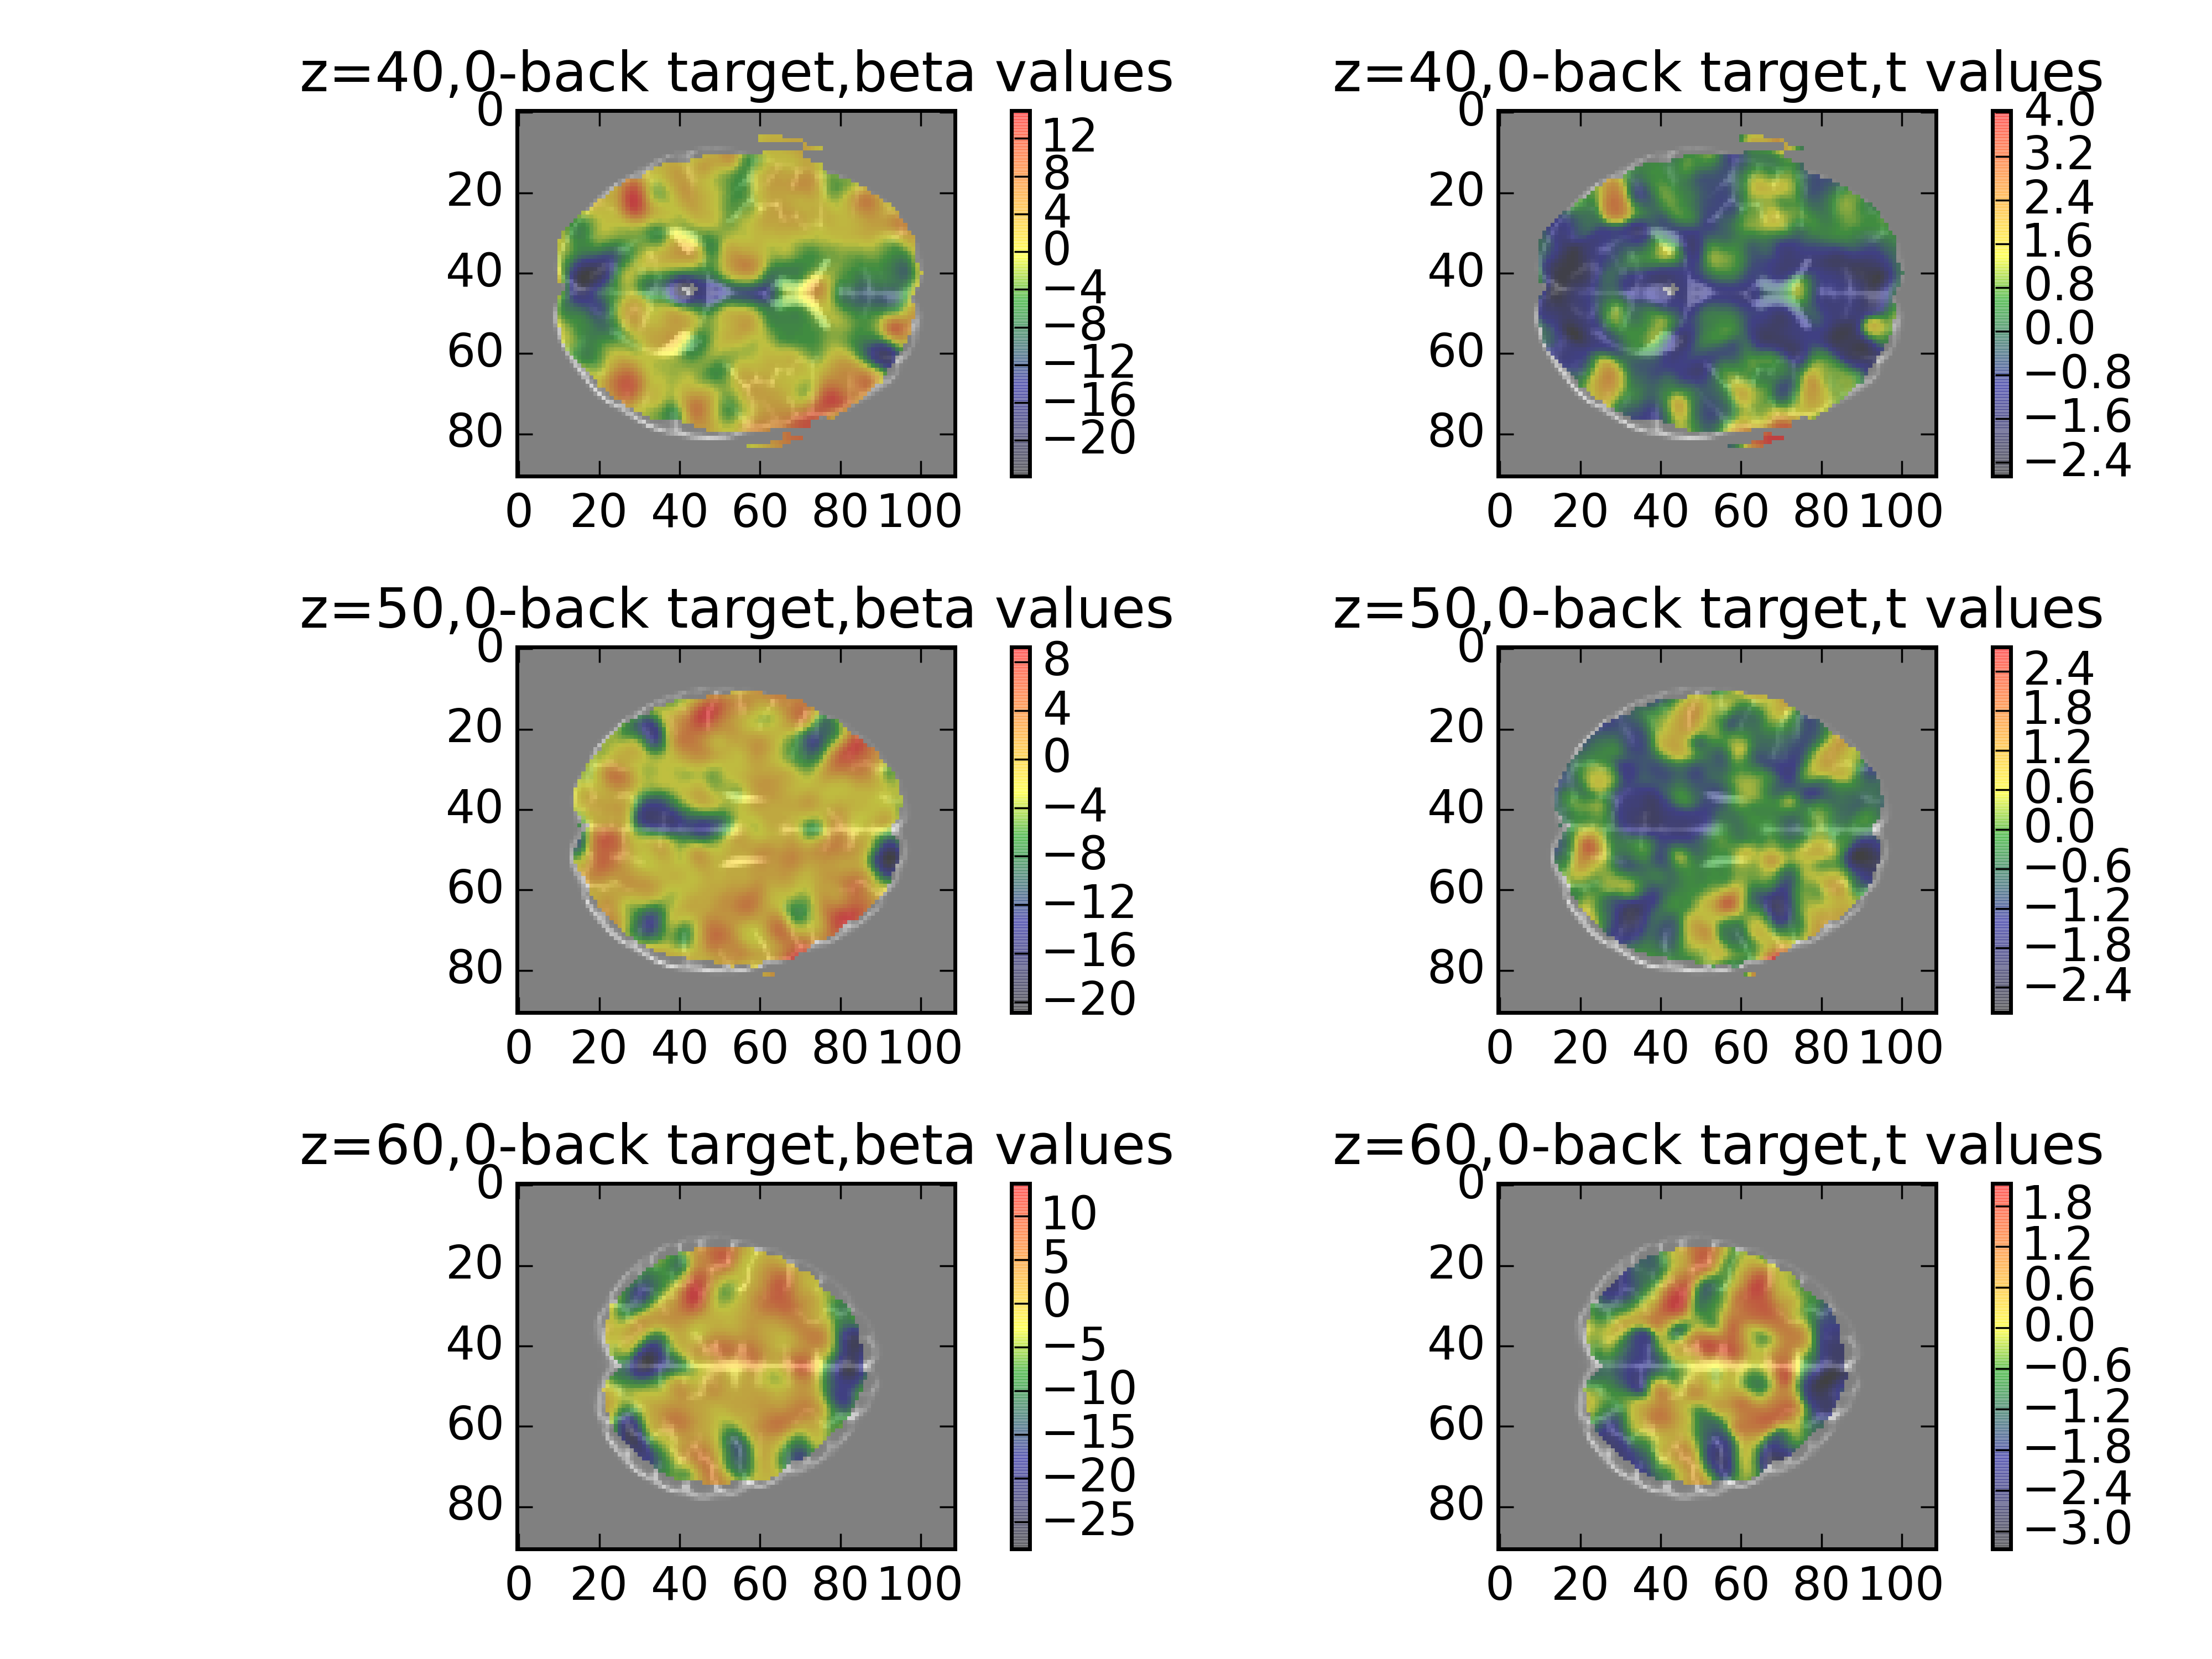
\includegraphics[scale=0.7]{../results/sub011_target_betas_0_back.png}
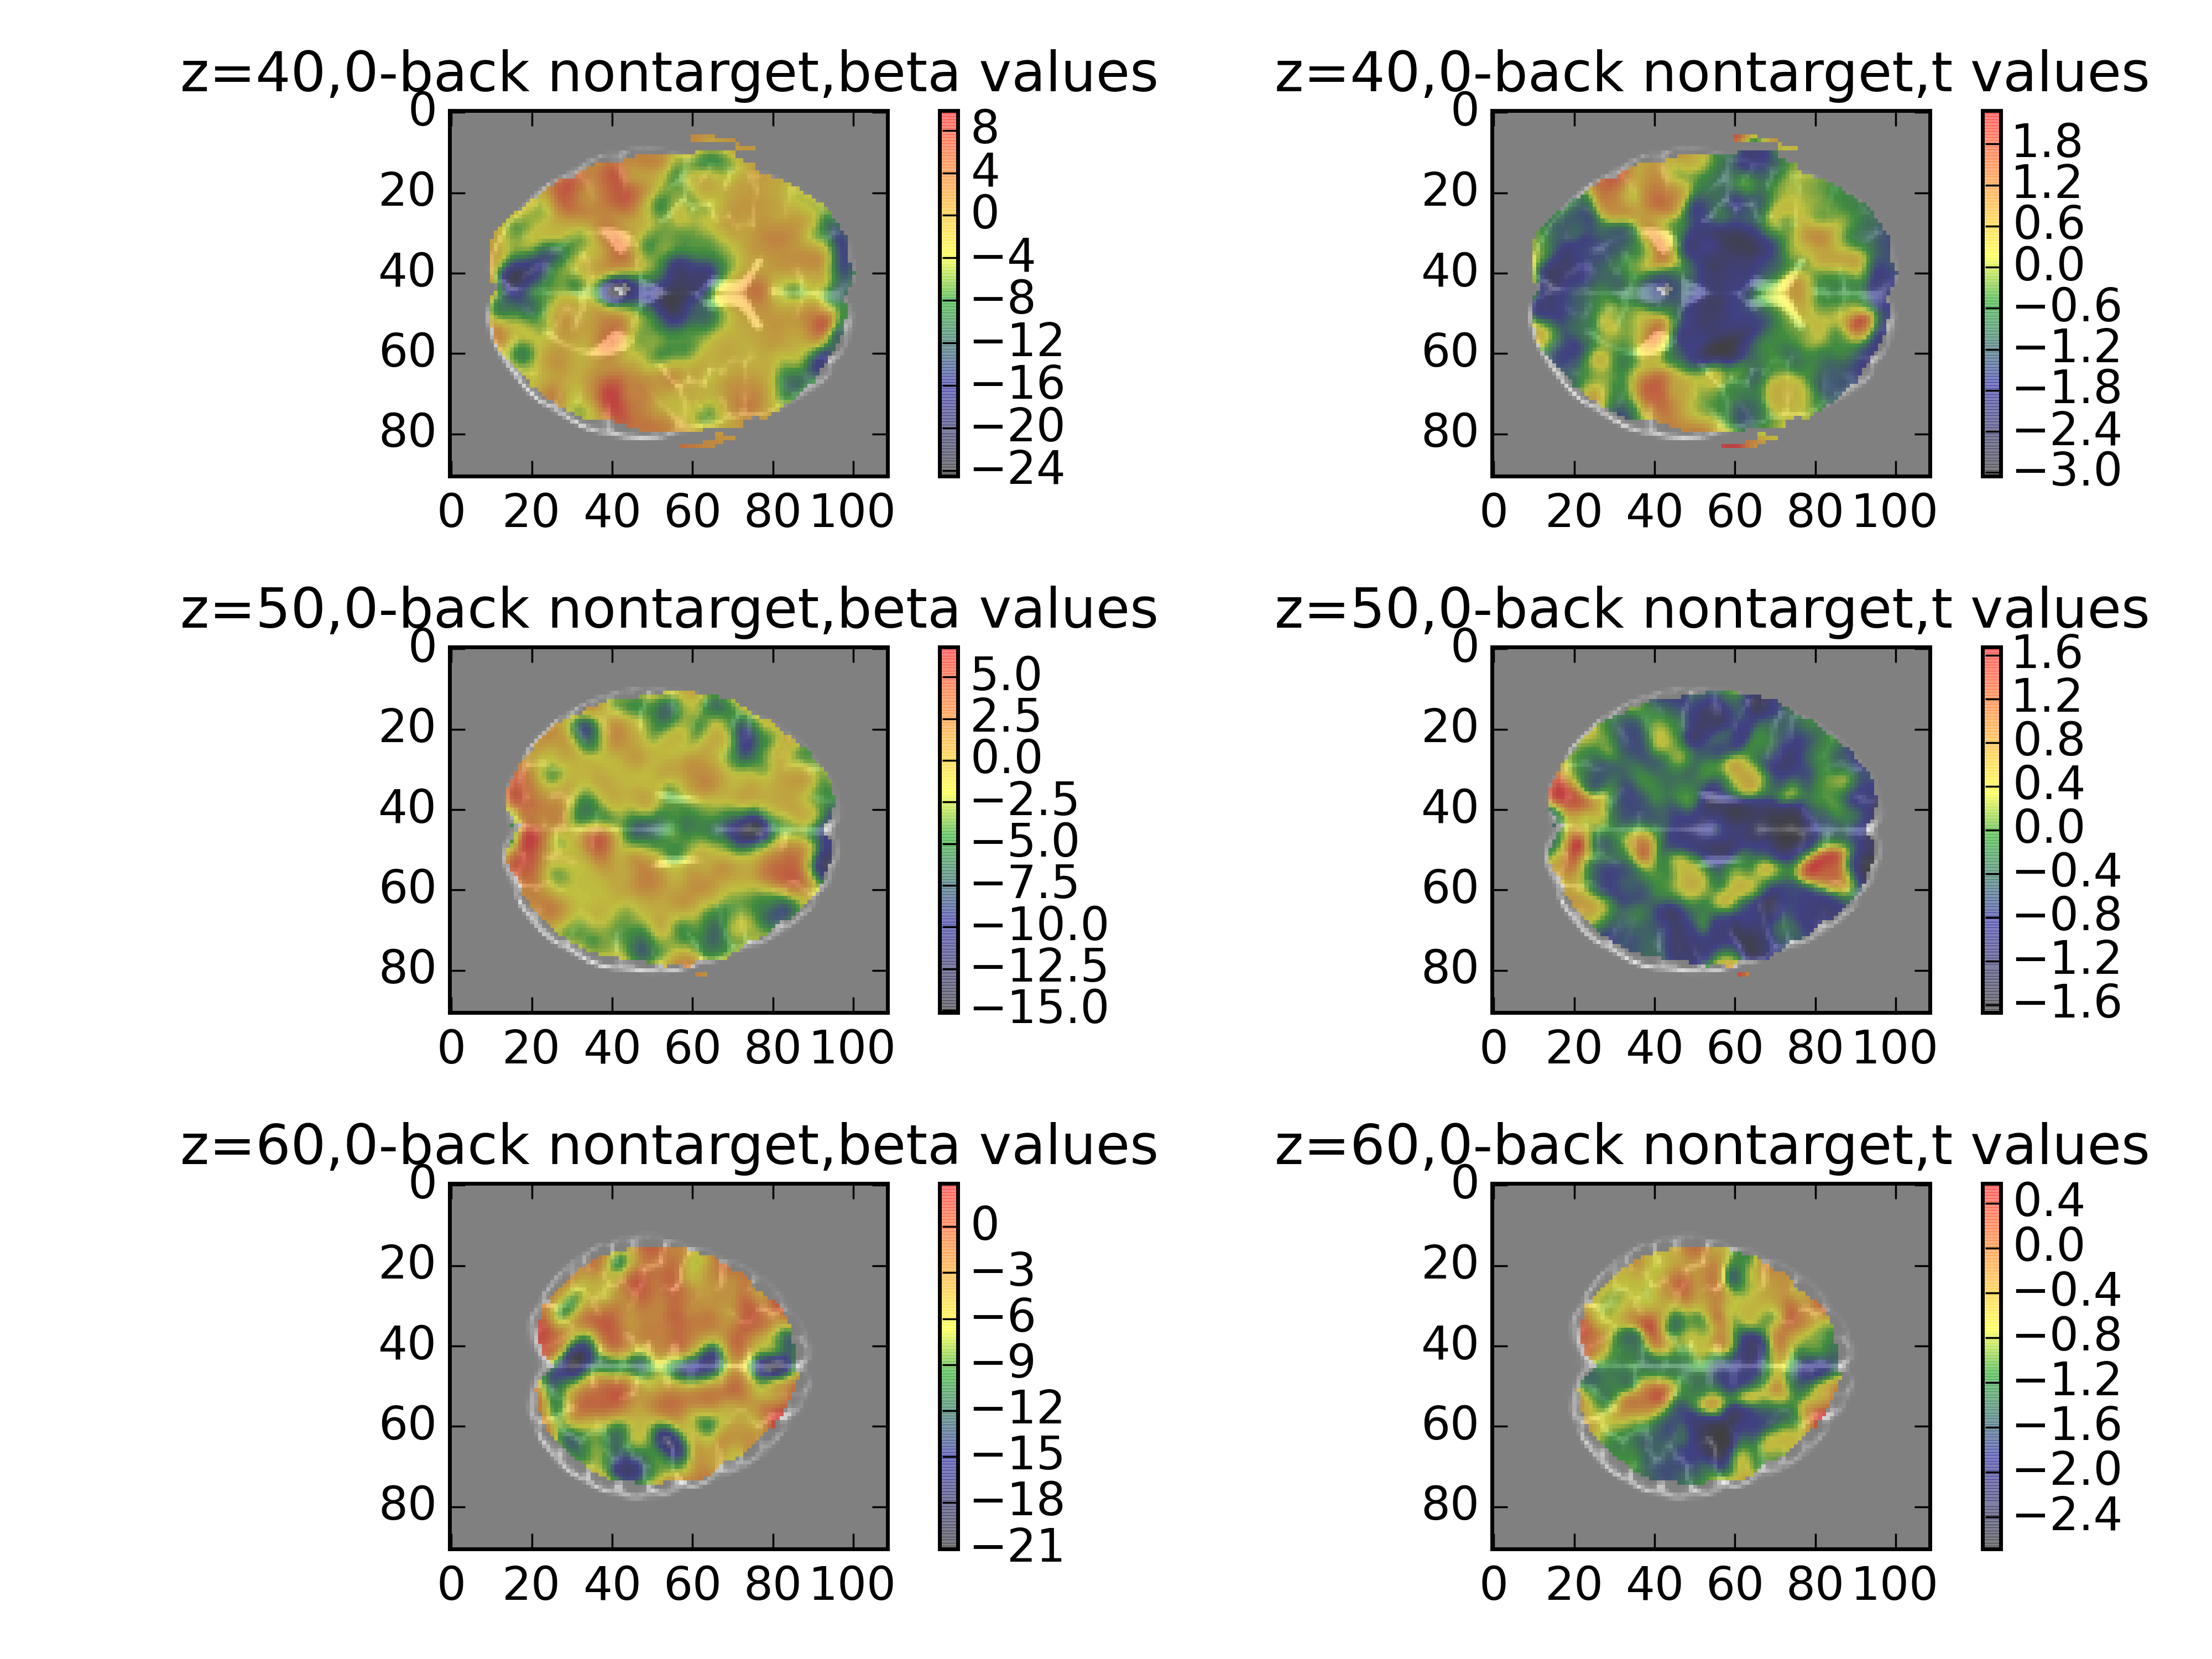
\includegraphics[scale=0.7]{../results/sub011_nontarget_betas_0_back.png}
\caption{Above: 0-back target beta values and t values from two-tailed t tests against the null hypothesis of $\beta = 0$; Below: non-target beta values and t values from two-tailed t tests against the null hypothesis of $\beta = 0$. Both are based on linear model for sub011 / 0-back, as discussed in the method section. The colors are plotted on the same scale for graphs in the same column.}
\end{figure}

As the 0-back task serves primarily as an object recognition task with respect to the activation it induces in the central nervous system, it would be expected that visual processing centers of the brain would be found to be most activated. As seen in both the beta maps and the associated t-value maps, there is considerable (and significant) activation of occipital cortex as well as various regions of the frontal cortex. In contrast to the responses observed with respect to the 2-back task presented below, the coefficient maps for the 0-back task for target images indicates fair amounts of activity across many regions of the brain, as would be expected of a general recognition test, whereas, in the 2-back task for target images, there is noticeably increased magnitudes in the activation of regions in the occipital cortex and in the frontal lobes, as would be expected of a task that involves working memory. It is worth noting that there is considerably less difference between the 0-back target vs. non-target activation patterns than between the 2-back target vs. non-target activation patterns, agreeing with the expectations based on psychological constructs such as working memory.

\begin{figure}
\centering
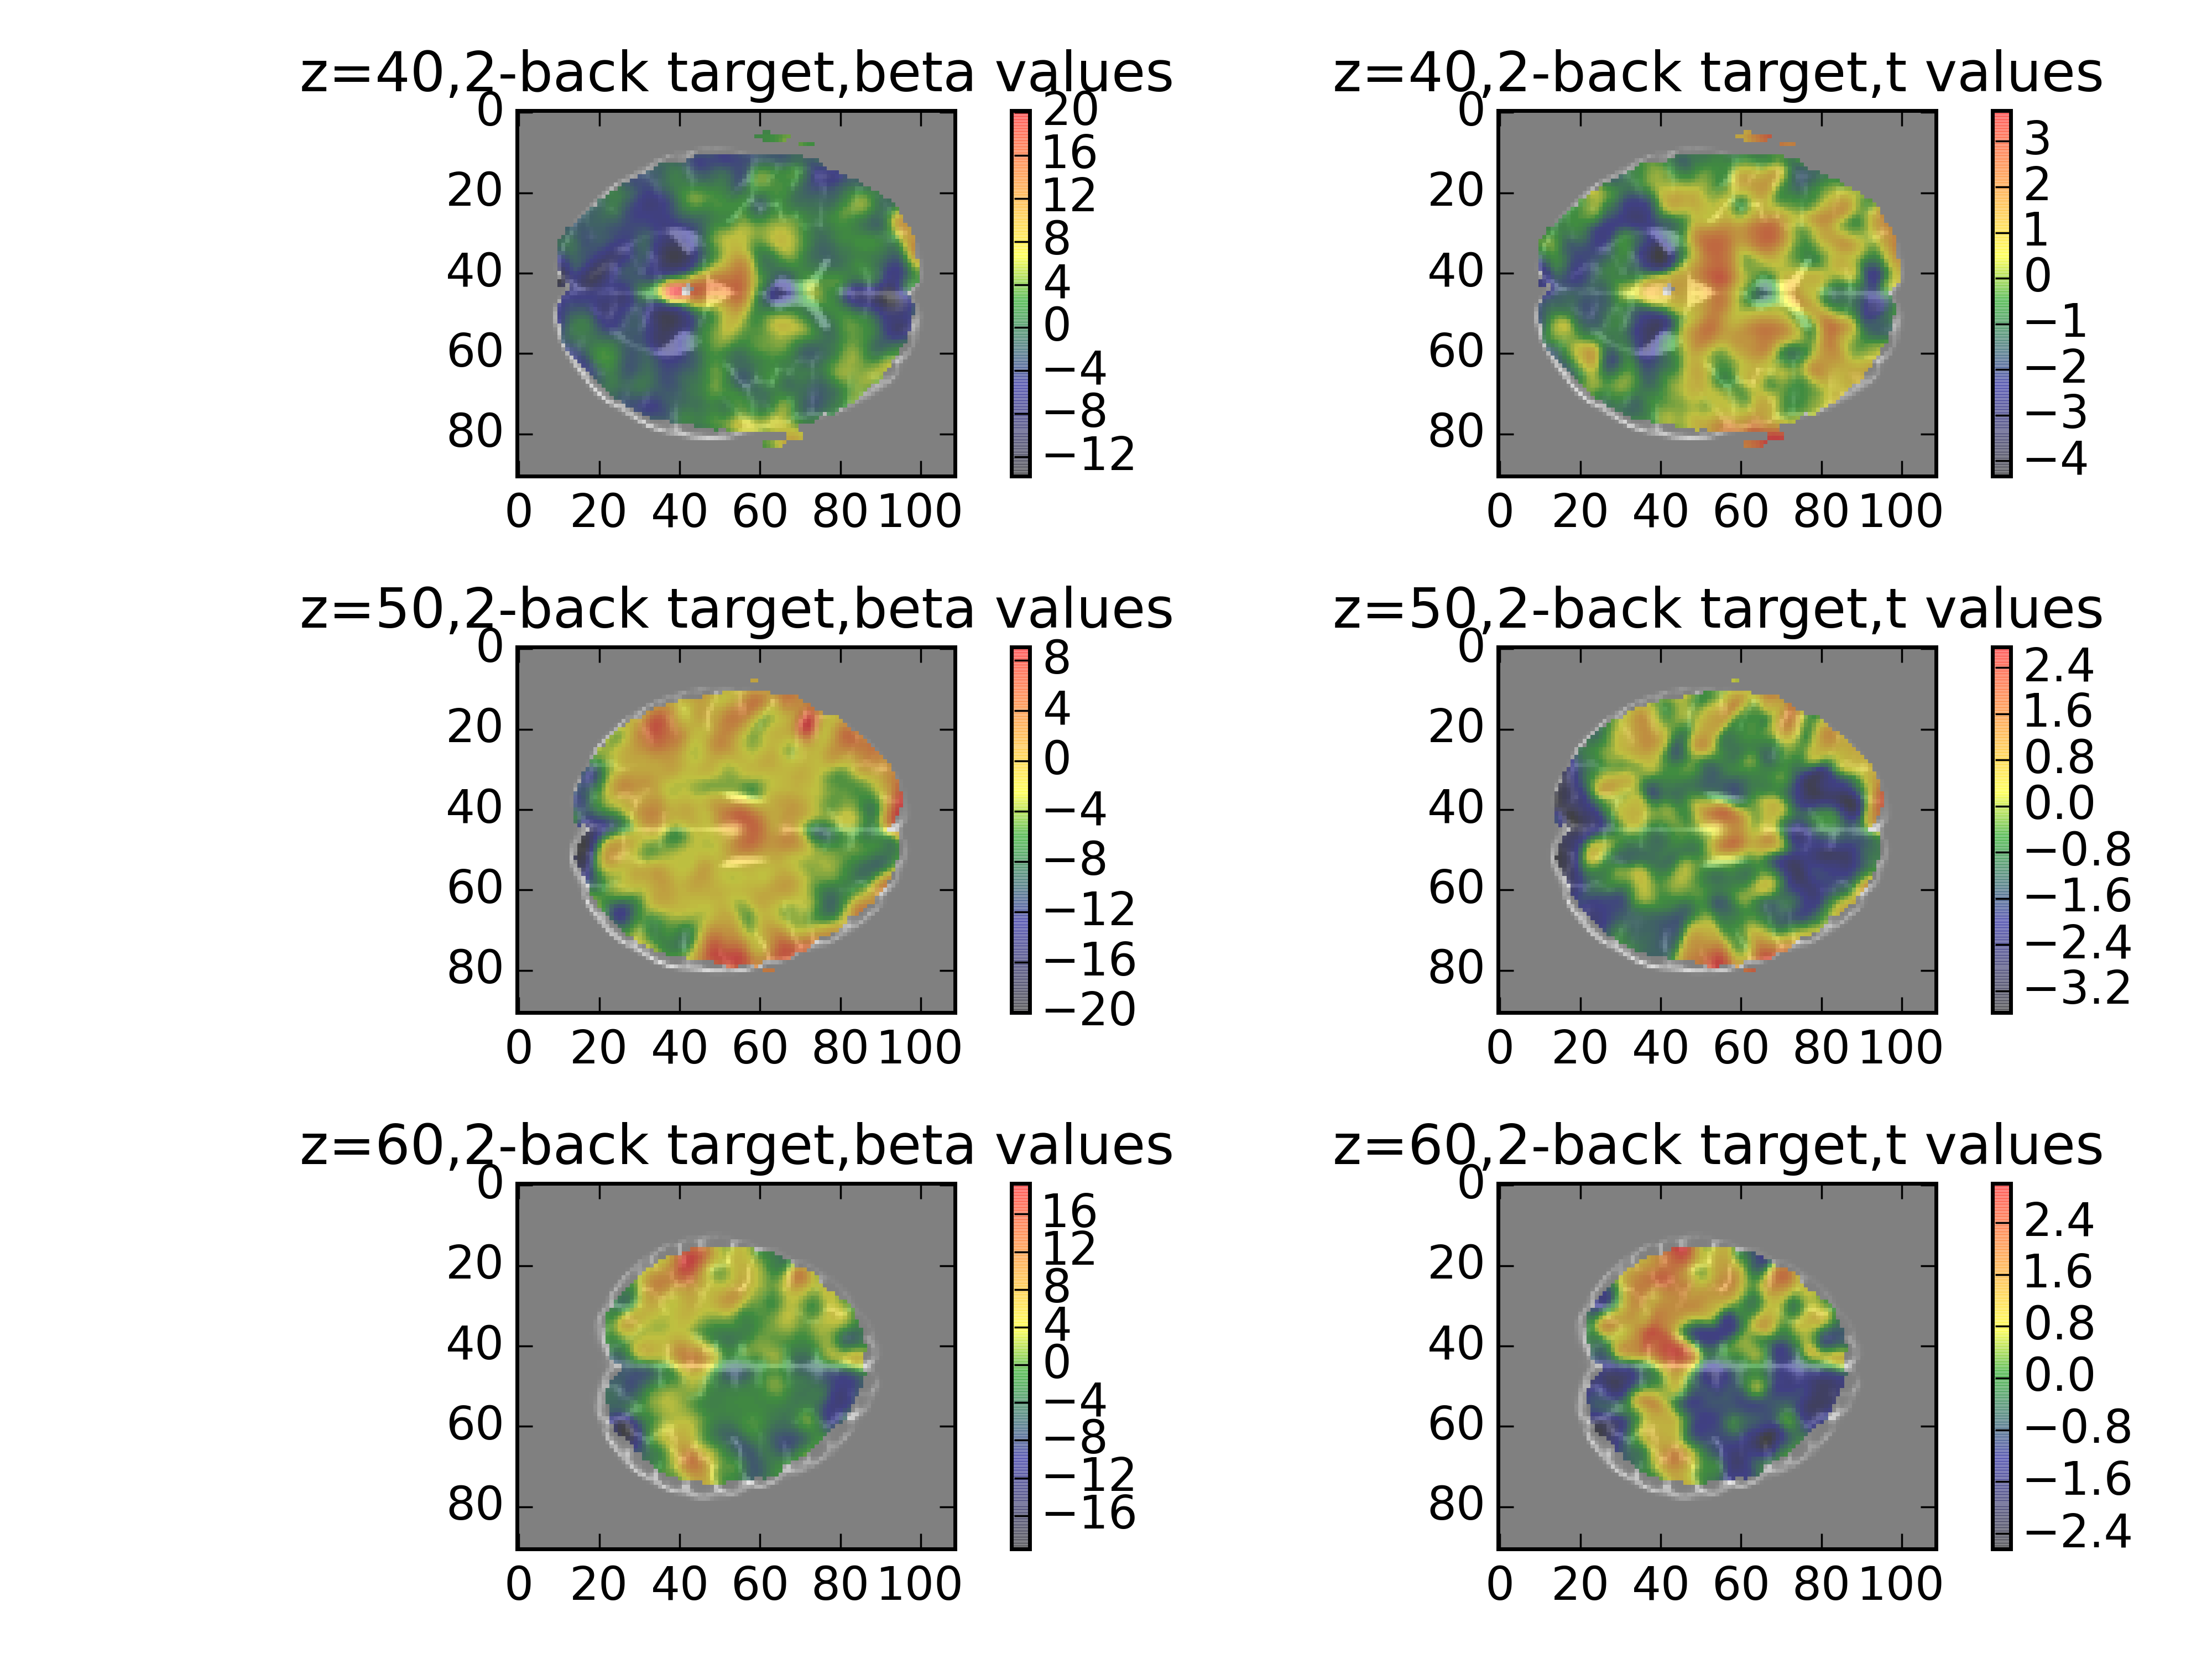
\includegraphics[scale=0.7]{../results/sub011_target_betas_2_back.png}
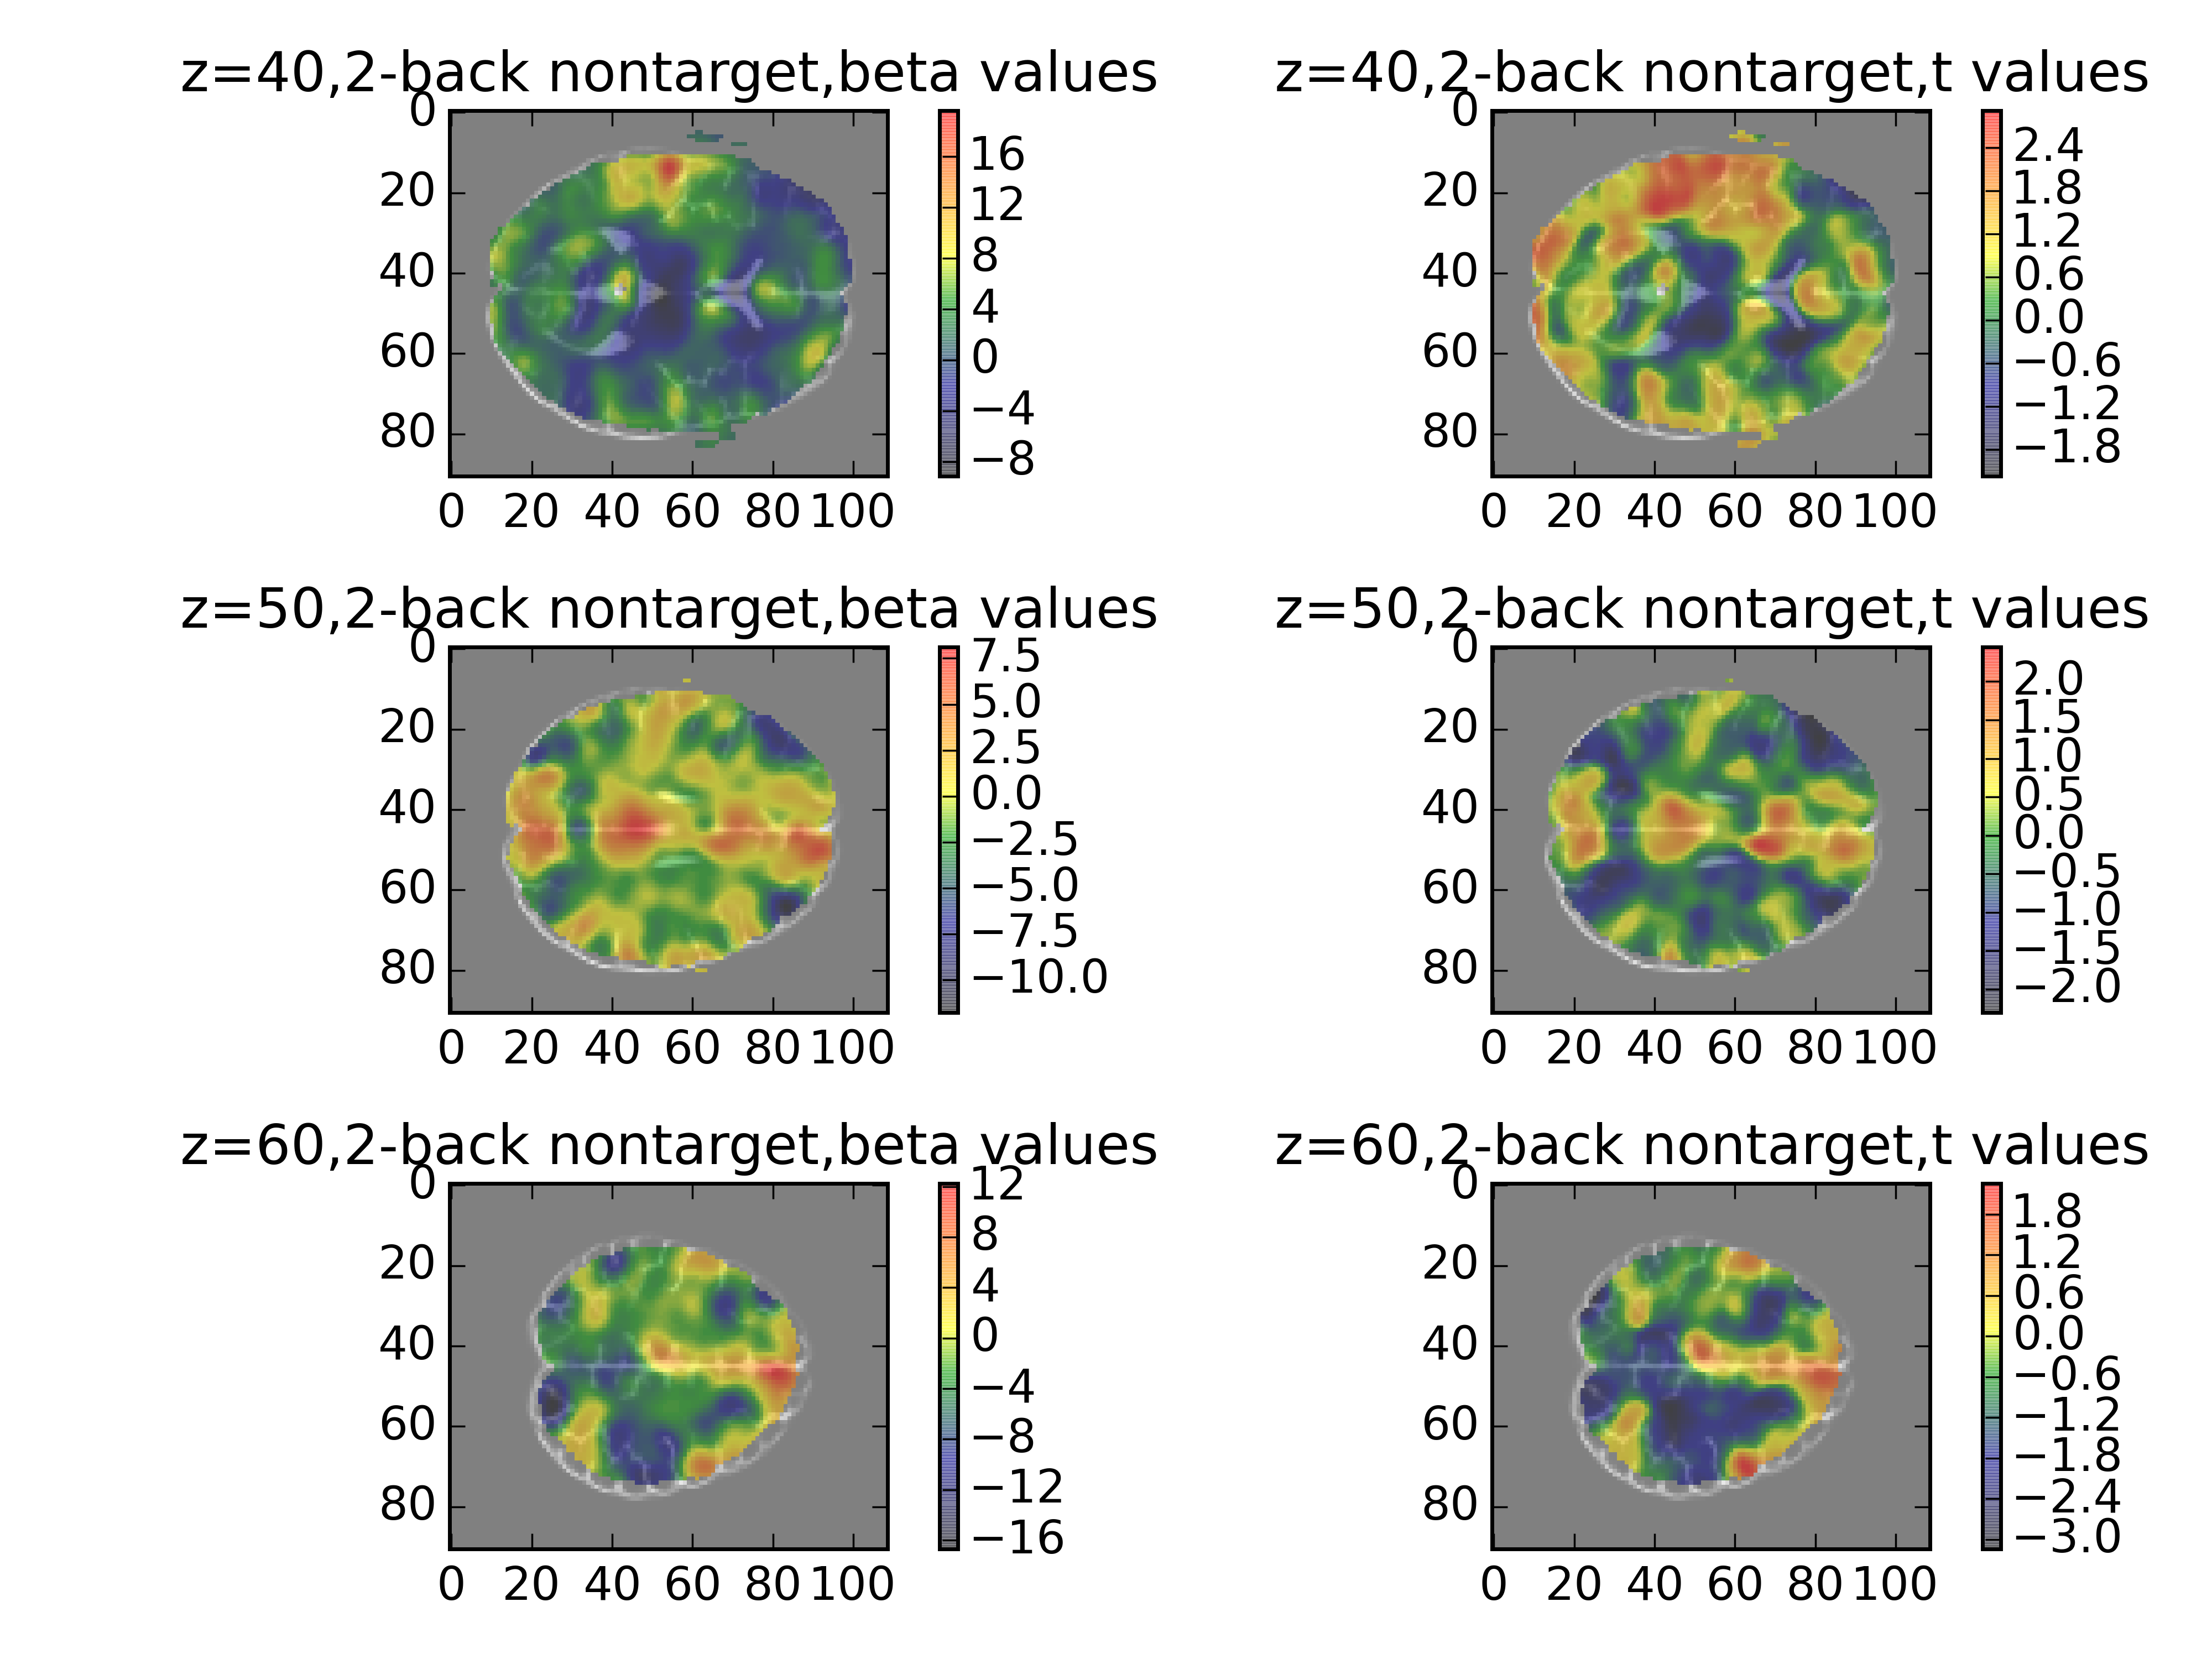
\includegraphics[scale=0.7]{../results/sub011_nontarget_betas_2_back.png}
\caption{Above: 2-back target beta values and t values from two-tailed t tests against the null hypothesis of $\beta = 0$; Below: non-target beta values and t values from two-tailed t tests against the null hypothesis of $\beta = 0$. Both are based on linear model for sub011 / 2-back, as discussed in the method section.}
\end{figure}

The two figures above display the observed activation patterns present in the 2-back task, which would be expected to activate regions of the prefrontal cortex more significantly than the 0-back task, on the basis that subjects must hold specific representations in memory in order to successfully complete this task. Furthermore, differences in the activation patterns between the target and non-target 2-back tests shows that the activation during the target task is less distributed, activating more specific regions, as opposed to the generalized activity created by undergoing the non-target 2-back task.

The non-target 2-back task activation patterns and associated t-value maps for the coefficients estimated from the linear model indicate that the non-target task generates activity across many regions of the central nervous system, in particular subregions in the frontal lobes (as seen in slice z=60) as well as numerous occipital and midbrain region activations (as seen in the slices z=50 and z=40). The many regions activated in the non-target 2-back analyses contrast sharply with the 2-back activations in the target group, as activations induced in the slices shown for that category are noticeably more focused in the occipital and frontal lobes.

The t-values associated with the coefficient estimates of the activation patterns in the 2-back target task show rather significant activation of frontal and midbrain regions, with these neural activations matching the more focused activation expected of a task more associated with inducing higher cognitive load. What is more, the differences in activation displayed by the two horizontal slices shown above illustrates how activation is distributed across the depths of the whole brain, in general activating frontal lobe regions associated with cognitive activity as well as occipital regions associated with visual task performance. With respect to the non-target activation patterns displayed in the slices shown below, the map of t-values indicate that activation is much more generally distributed across the brain in the non-target 2-back task, as would be expected of an error-based neural process.

\subsection{Connectivity Analysis}

\begin{figure}[H]
\centering
\includegraphics[scale=0.7]{../results/inter_network_connectivity_plot.png}
\caption{The connectivity plot comparing schizophrenics (SCZ) and controls (CON) between networks. For visual comparison, the CON group and SCZ group are interleaved in order to show results for the same network-nework pair side by side.}
\end{figure}

We performed the analysis on 20 subjects\footnote{Subject numbers listed on the OpenfMRI project: 011, 012, 015, 035, 036, 037, 010, 013, 014, 021, 022, 038, 007, 009, 017, 031, 006, 008, 018, 024}, including 12 SCZ (6 schizophrenias and 6 schizophrenia siblings) and 8 CON (4 controls and 4 control siblings). As shown in the figure above, the individuals with schizophrenia and their siblings (SCZ) showed an overall reduction in connectivity between the cognitive control networks as compared to CON, as indicated in the box plots of the correlations between networks for CON and SCZ. Because of the various confounding factors typical in experiments involving schizophrenia patients, a more detailed discussion of the results can be found in the discussion section.  
To statistically quantify the group-level differences, permutation tests were conducted in different pairs of networks as outlined in the method section. We found that all of the test rejected the null hypothesis, suggesting that the mean network-network correlation values of SCZ groups are significantly less than those of CON group \footnote{The results were generated from our analysis scripts, and can be found in the results folder at \textit{connectivity\_permutation\_result.csv}}.

Within-network correlations are not within the scope of our analysis, but a graph showing the results for within-network correlations, included in the appendix, showed similar reductions.


\section{Discussion}

Previous studies concluded that there is reduced distal connectivity for individuals with schizophrenia, especially between the FP and CER networks and the CO and CER networks \cite{repovs2011, repovs2012}. However, the two results are not comparable in the following ways: (1) we use a smaller dataset of 20 subjects versus 102 subjects used in the reference paper, and (2) in the reference papers, many more nuisance regressors were removed from the BOLD time series. We only removed a few common noise regressors outlined in the methods section above. We obtained results similar to the previous work and provided similar evidence that schizophrenia reflects a disconnection syndrome.

As presented so far, the analyses presented show that connectivity differences
between schizophrenics and biologically matched controls can be isolate. In the
examination of the effects of schizophrenia on connectivity, the authors of the
original paper used schizophrenics and (as a control group) healthy siblings so
as to ensure that the experimental and control groups matched on physiological
and genetic factors. This approach ensures that any observed differences in the
fMRI connectivity analysis performed are not related to biological differences
that may be irrelevant (e.g., genetic differences between individuals). Despite
the added rigor provided by adopting this approach, more could have been done to
ensure that any observed connectivity differences are not the direct results of
behavioral or lifestyle differences between members of the two groups \cite{gur2010functional}. 

Since the researchers did not denote such features as whether subjects were smokers or the
degree to which subjects fidgeted while undergoing scanning, there are potential
variations (possibly, though indirectly, attributable to schizophrenia) between
members of the two groups, reducing the conclusions that may be drawn from the
connectivity results that we present. In particular, the effects of lifestyle
choices on neural connectivity as measured by fMRI have been documented in the
case of schizophrenics -- that is, it has been found that schizophrenia promotes
lifestyle choices, such as a tendency towards smoking, that can alter neural
connectivity \cite{leyba2008smoking}. Thus, as we are only able to take into 
account baseline features that were documented by the original researchers in 
our analyses, there are a number of limitations caused by missing information. 
We believe that the issues in interpretability of the conclusions we present 
are most clearly captured in the simplified directed acyclic graph of potential 
confounding provided in the diagram that follows. \\[5pt]

\begin{figure}[H]
\centering
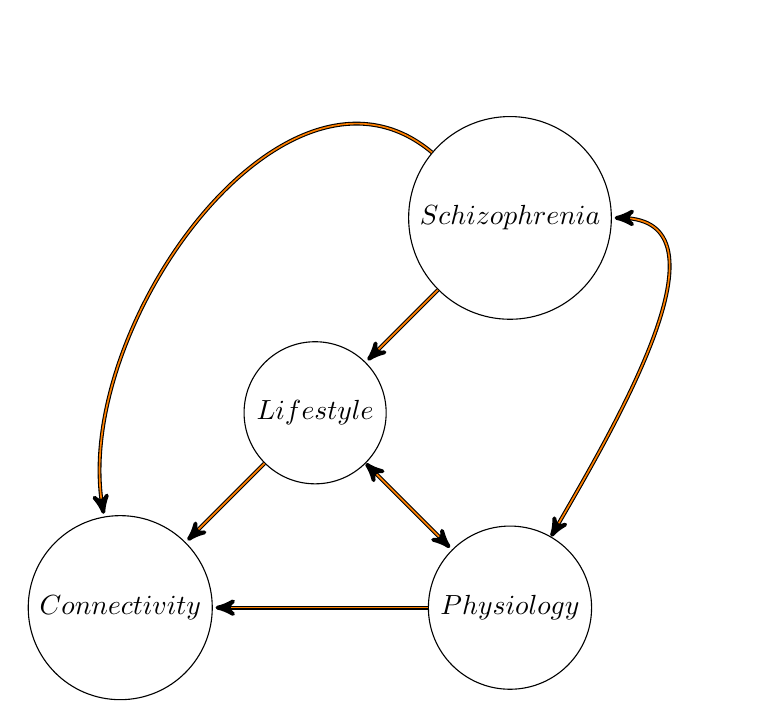
\begin{tikzpicture}[>=stealth',shorten >=1pt,node distance=3.5cm,on grid,initial/.style    ={}]
  \node[state]          (Connectivity)                        {$Connectivity$};
  \node[state]          (Lifestyle) [above right =of Connectivity]    {$Lifestyle$};
  \node[state]          (Schizophrenia) [above right =of Lifestyle]    {$Schizophrenia$};
  \node[state]          (Physiology) [below right =of Lifestyle]    {$Physiology$};
\tikzset{mystyle/.style={->,relative=false,double=orange}} 
\tikzset{every node/.style={fill=white}} 
\path (Schizophrenia)     edge [mystyle]    (Lifestyle)
      (Lifestyle)	edge [mystyle]	  (Connectivity)
      (Physiology)	edge [mystyle]	 (Connectivity);
\tikzset{mystyle/.style={<->,double=orange}}   
\path (Lifestyle)     edge [mystyle]    (Physiology);
\tikzset{mystyle/.style={->,relative=false,in=100,out=500,double=orange}}
\path (Schizophrenia)     edge [mystyle]   (Connectivity); 
\tikzset{mystyle/.style={<->,relative=false,in=0,out=60,double=orange}}
\path (Physiology)     edge [mystyle]   (Schizophrenia); 
\end{tikzpicture}
\caption{Directed acyclic graph illustrating potential for confounding}
\end{figure}

\bibliography{report}

\newpage
\appendix

\section{APPENDIX I - Results for Within-Network Correlations}

\begin{figure}[H]
\centering
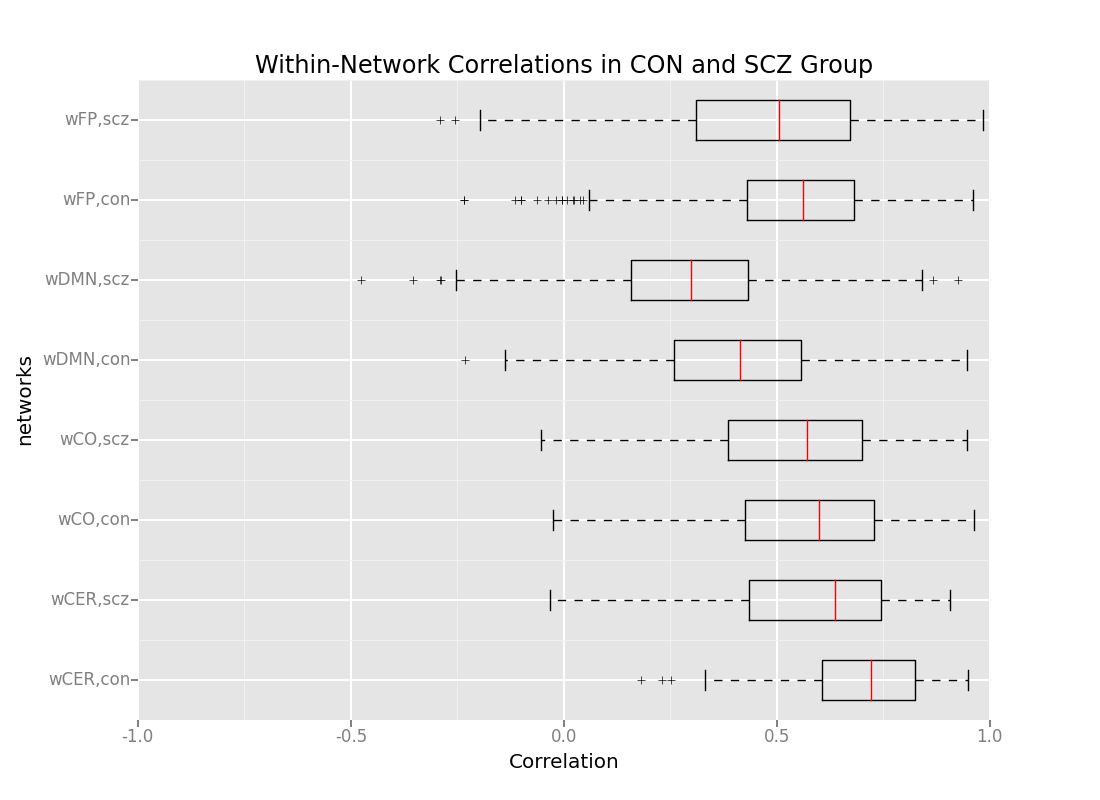
\includegraphics[scale=0.7]{../results/within_network_connectivity_plot.png}
\caption{The connectivity plot comparing schizophrenics (SCZ) and controls (CON) within networks. For visual comparison, the CON group and SCZ group are interleaved in order to show results for the same network side by side.}
\end{figure}

\section{APPENDIX II - Exploratory Data Analysis}

\subsection{Data Fetching and Preprocessing}

Except for Extended RMS analysis, the standard preprocessed BOLD images were used. They were already preprocessed with (1) motion correction (co-registration in time to partially correct for movement during the run and between runs); (2) temporary high-pass filtering to remove low frequency drifts and/or noise; and (3) registration to a standard anatomical template (the MNI template). In EDA, we detected several extended root-mean-square (RMS) outliers for the BOLD datasets. This further justified the need for temporary smoothing. For our preprocessing steps, first five images of each run were removed to allow measurements to achieve steady state. Each image was passed through a gaussian filter of $\sigma=2$. This spatial smoothing approach assumes that fMRI data inherently show spatial correlations due to functional similarities of adjacent brain regions.
\subsection{Extended Root Mean Square (RMS) Difference Outliers}

BOLD images were known to contain a sudden widespread shift in signals caused by hardware issues. We
wanted to confirm the hypothesis by finding RMS difference outliers using the inter-quartile range (IQR).

\begin{figure}[H]
\centering
\includegraphics[scale=0.5]{../results/sub011_task011_extended_RMS_outliers.png}
\caption{The extended RMS outliers for the BOLD images for sub011, 0-back}
\end{figure} 

\subsection{Correlations with Baseline Functions}

For this analysis, the images were smoothed and the first two Principal Componenets were
removed. This set of methods aimed to produce images identifying the regions which showed
significant signal change in response to the task. The analysis was done by calculating 
correlation coefficients (r) between the bold signal along the time course and a reference
waveform, for each voxel. The reference waveform was extracted from one condition file.
Condition file 003 was chosen because while it did not contain all stimuli presented to the
subject, such as start and done cues, it included all target and non-target events and this
was thought to be sufficient to elicit functional differences of the brain during the run. 
A high value of the correlation coefficient indicated that fluctuation of the signal in 
the locale of the brain was task-dependent, hence activated by the task. 

For a bold signal X, and a reference waveform Y, the correlation coefficient is
calculated as below.

\begin{equation}
r = \frac{\Sigma_{i=1}^{n}  ( X-\bar{X}) ( Y-\bar{Y})}{\sqrt{ \Sigma_{i=1}^{n} (
    X-\bar{X} ) ^2 \Sigma_{i=1}^{n} ( Y-\bar{Y})  ^2 }}
\end{equation}

The two methods were differentiated by two types of reference
waveforms: (1) square wave using on-off neural prediction from condition file
(SW method), and (2) a convolved function on neural predictions with a gamma
haemodynamic response function (HRF) (CF method).

Here, the two types of analysis were compared. By comparing
the activated regions under square wave time course (left) and convolved time
course (right), we could see that compared to SW method, the CR method gives 
more reasonable and detailed results.

\begin{figure}[H]
\centering
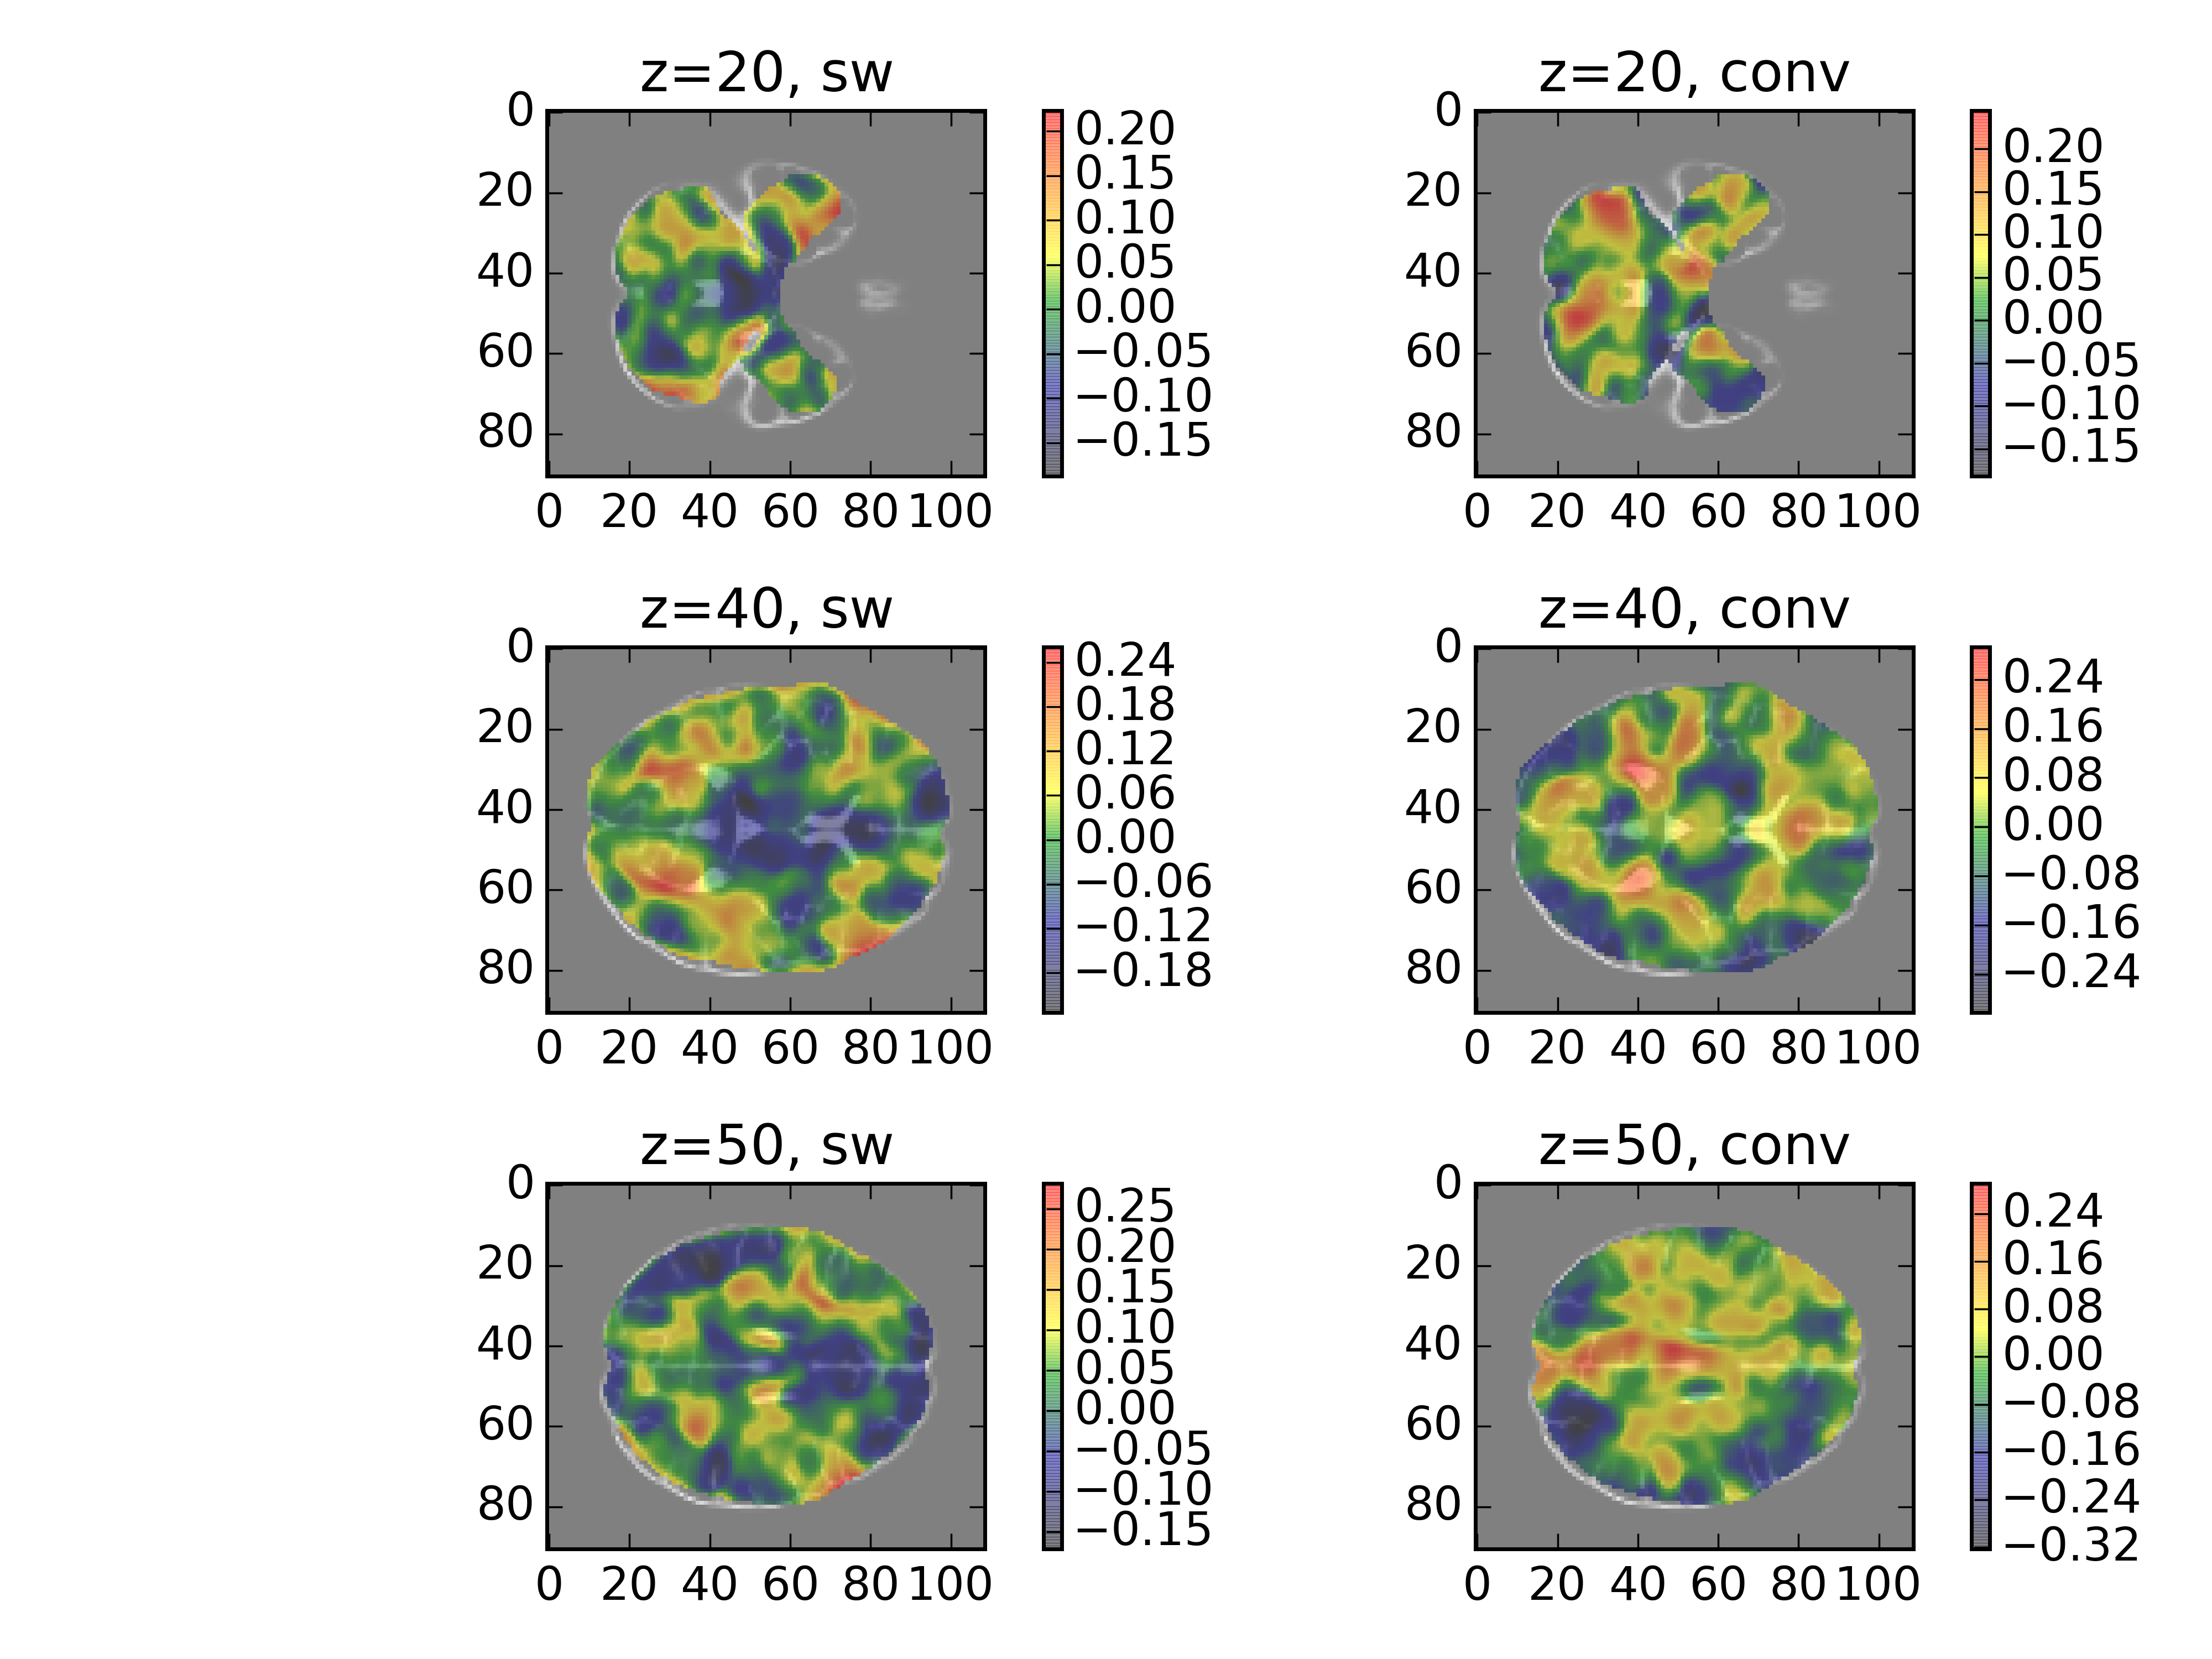
\includegraphics[scale=0.7]{../results/sub011_voxel_wise_correlation_across_methods.png}
\caption{Voxel-wise correlations for square-wave and gamma baseline functions, sub011, 0-back, cond003.}
\end{figure} 

\subsection{Clustering with K-Means}

K-means clustering is an unsupervised technique which aims to partition n
observations into k clusters based on a feature set of n features. Each
observation is classified into the cluster with the nearest mean. In our case,k was
chosen to be 6. Input to k-means clustering followed the same treatment as discussed
in the Linear Model section of the paper. Standard fMRI data was and the first two 
Principal Components were removed following the analysis in the Linear Model section 
of the paper. After that, it was spatially smoothed with gaussian kernel
of $sigma=2$. The rationale of removing the first two Principal Components was to
remove differences caused by anatomical or other noise features as much as possible, in
the hope that k-means can cluster the brain to functional regions.

We did not involve the condition files in the clustering. This was because during
the same run, the time courses in the same region of the brain were subjected to the
same functional influences. Hence, k-means should be able to detect differences in
patterns of the time courses between regions.

\begin{figure}[H]
\centering
\includegraphics[scale=0.7]{../results/sub011_kmeans_6_groups_smoothed.png}
\caption{K-means result for $k=6$ on smoothed standard fMRI data after removal of first two Principal Components, sub011, 0-back. Note that the clustering across different slices appears to match the underlying neurobiology rather well -- for example, the yellow cluster of voxels includes both frontal and occipital regions, both being regions activated in the visual working memory tasks considered in this analysis.}
\end{figure} 

\section{APPENDIX III - Linear Model Noise Regressors}

\begin{figure}[H]
\centering
\includegraphics[scale=0.7]{../results/sub011_0_back_noise_regressors_betas_map.png}
\caption{Beta and t values for some of the noise regressors included in the linear model for sub011, 0-back.}
\end{figure} 

\end{document}
















